\documentclass[12pt,spanish,Letterpaper,openany]{book}
\usepackage{lmodern}
\usepackage{setspace}
\setstretch{0.85}
\usepackage{amssymb,amsmath}
\usepackage{ifxetex,ifluatex}
\usepackage{fixltx2e} % provides \textsubscript
\ifnum 0\ifxetex 1\fi\ifluatex 1\fi=0 % if pdftex
  \usepackage[T1]{fontenc}
  \usepackage[utf8]{inputenc}
\else % if luatex or xelatex
  \ifxetex
    \usepackage{mathspec}
  \else
    \usepackage{fontspec}
  \fi
  \defaultfontfeatures{Ligatures=TeX,Scale=MatchLowercase}
    \setmainfont[Scale=1.0, HyphenChar=None]{Corbel}
    \setsansfont[]{Corbel}
    \setmonofont[Mapping=tex-ansi]{Corbel}
\fi

\makeatletter
\renewcommand\mainmatter{\clearpage\@mainmattertrue\pagenumbering{arabic}}
\renewcommand\frontmatter{\clearpage\@mainmatterfalse\pagenumbering{arabic}}
\renewcommand\backmatter{\clearpage\@mainmatterfalse}
\makeatother

%\usepackage{etoolbox}
%\makeatletter
%\patchcmd{\@smemmain}{\cleardoublepage}{\clearpage}{}{}
%\patchcmd{\@smemmain}{\cleardoublepage}{\clearpage}{}{}
%\patchcmd{\@smemfront}{\cleardoublepage}{\clearpage}{}{}
%\patchcmd{\@smemfront}{\cleardoublepage}{\clearpage}{}{}
%\makeatother

\setlength{\parindent}{0em}

\usepackage{graphicx}
\usepackage{booktabs}
\usepackage{multicol}
\usepackage{doc}
\usepackage{float}
\usepackage{tcolorbox} 
\usepackage{lipsum}
\usepackage{tikz}
\usepackage{nonfloat}

\usepackage{pdfpages}

\usepackage[
contents={},
opacity=1,
scale=1.5,
color=blue!90
]{background}
\usepackage{lipsum}
\usepackage{ifthen}

\usepackage{xcolor}
\usepackage[pagestyles]{titlesec}

\renewpagestyle{plain}[\normalsize\sffamily\bfseries\slshape]{
  \setfoot{}{\color{black}{\thepage}}{}}

\newpagestyle{myps}[\normalsize\sffamily\bfseries\slshape]{
  \setfoot{}{\color{black}{\thepage}}{}}
  
\pagestyle{myps}


\usepackage{framed}
\definecolor{colorlinetitle}{HTML}{a87e00}%{a87e00}%
\definecolor{textlinetitle}{HTML}{061769}%{061769}%{061769}%
\definecolor{fondo}{HTML}{041d57}%
\definecolor{newfondo}{HTML}{3d0718}%
\colorlet{shadecolor}{fondo!81!}


% use upquote if available, for straight quotes in verbatim environments
\IfFileExists{upquote.sty}{\usepackage{upquote}}{}
% use microtype if available
\IfFileExists{microtype.sty}{%
\usepackage{microtype}
\UseMicrotypeSet[protrusion]{basicmath} % disable protrusion for tt fonts
}{}
\usepackage[inner=12.7mm,outer=12.7mm,top=24mm,bottom=20mm]{geometry}
\usepackage{hyperref}
\hypersetup{unicode=true,
            pdftitle={Revista digital de la unidad de prácticas de ingeniería y EPS},
            pdfauthor={Unidad de Prácticas de Ingeniería y Ejercicio Profesional Supervisado},
            pdfborder={0 0 0},
             breaklinks=true,
	  linkcolor=black,
	  urlcolor=darkgray}
\urlstyle{same}  % don't use monospace font for urls
\ifnum 0\ifxetex 1\fi\ifluatex 1\fi=0 % if pdftex
  \usepackage[shorthands=off,main=spanish]{babel}
\else
  \usepackage{polyglossia}
  \setmainlanguage[]{spanish}
\fi
\usepackage{natbib}
\bibliographystyle{apalike}
\usepackage{longtable,booktabs}
\IfFileExists{parskip.sty}{%
\usepackage{parskip}
}{% else
\setlength{\parindent}{0pt}
\setlength{\parskip}{6pt plus 2pt minus 1pt}
}
\setlength{\emergencystretch}{3em}  % prevent overfull lines
\providecommand{\tightlist}{%
  \setlength{\itemsep}{0pt}\setlength{\parskip}{0pt}}
\setcounter{secnumdepth}{5}
% Redefines (sub)paragraphs to behave more like sections
\ifx\paragraph\undefined\else
\let\oldparagraph\paragraph
\renewcommand{\paragraph}[1]{\oldparagraph{#1}\mbox{}}
\fi
\ifx\subparagraph\undefined\else
\let\oldsubparagraph\subparagraph
\renewcommand{\subparagraph}[1]{\oldsubparagraph{#1}\mbox{}}
\fi

%%% Use protect on footnotes to avoid problems with footnotes in titles
\let\rmarkdownfootnote\footnote%
\def\footnote{\protect\rmarkdownfootnote}


  \title{Revista digital de la unidad de prácticas de ingeniería y EPS}
    \author{Unidad de Prácticas de Ingeniería y Ejercicio Profesional Supervisado}
      \date{2025-09-19}

% no title page
\AtBeginDocument{\let\maketitle\relax}

\usepackage{caption2}
\captionsetup{%
labelsep=colon,%
font={footnotesize},%
aboveskip=0.4\baselineskip,%
belowskip=0\baselineskip,% deve essere 0 perché regolo lo spazio dal testo con \intextsep
}%

\usepackage{booktabs}
\usepackage{longtable}

\usepackage{indentfirst}
\setlength{\parindent}{1em}
\usepackage{enumitem}
\setlist[itemize]{labelindent = \parindent, leftmargin=*}

%\usepackage{framed,color}
%\definecolor{shadecolor}{RGB}{248,248,248}

\renewcommand{\textfraction}{0.05}
\renewcommand{\topfraction}{0.8}
\renewcommand{\bottomfraction}{0.8}
\renewcommand{\floatpagefraction}{0.75}

\renewcommand{\chaptername}{Artículo}
\addto\captionsspanish{\renewcommand{\chaptername}{Artículo}}
\addto\captionsspanish{\renewcommand{\contentsname}{Índice general}}


\frenchspacing
\tolerance=5000
\multicoltolerance=3000 

\raggedbottom
\raggedcolumns

\setlength{\columnsep}{1em}
%We want a rule between columns.
%\setlength\columnseprule{.4pt}

%Tambien queremos asegurarnos de que un nuevo entorno multicols 
%encuentre suficiente espacio en la parte inferior de la pagina.
\setlength\premulticols{6\baselineskip}

%Al equilibrar columnas, ignoramos las soluciones que son 
%demasiado malas. Ademas, si la ultima columna es demasiado mala, 
%la tipeamos sin estirar.
\setcounter{columnbadness}{7000}
\setcounter{finalcolumnbadness}{7000}

\newcommand{\prefacetitlecommand}%
{\titleformat{\chapter}[display]%
{\bfseries\large\color{colorlinetitle}}%
{\relax}%
{0ex}%
{{\titlerule[1.2pt]}\filright\color{textlinetitle}}[\color{colorlinetitle}\vspace{0.5ex}{\titlerule[1.2pt]}]%
}


\newcommand{\articletitlecommand}%
{\titleformat{\chapter}[display]%
{\bfseries\tiny\raggedright\color{white}}%
{\relax}%
{0ex}%
{}[\color{white}\vspace{0ex}{\titlerule[0pt]}]%
}



\newcommand{\sectionCenter}%
{\titleformat{\section}[block]%
{\bfseries\large\color{textlinetitle}\filcenter}%
{\relax}%
{0ex}%
{\empty}%
}


\newcommand{\sectionRight}%
{\titleformat{\section}[block]%
{\bfseries\large\color{textlinetitle}}%
{\relax}%
{0ex}%
{\empty}%
}


\newcommand{\subsectionRight}%
{\titleformat{\subsection}[block]%
{\bfseries\normalsize\color{textlinetitle}}%
{\relax}%
{0ex}%
{\empty}%
}

\usepackage{titletoc}
\titlecontents{chapter}[3em]
{\vspace{5mm}}
{\normalsize\contentslabel[\color{textlinetitle}\thecontentslabel]{2em}\color{black}\itshape\normalsize}
{\color{black}\itshape\normalsize}
{\color{colorlinetitle}\titlerule*[.3pc]{.}\color{black}\contentspage}

\newcommand{\tcolorboxcommand}{\begin{tcolorbox}[sharp corners=uphill, colback=newfondo, colframe=newfondo, arc=6mm, boxrule=0mm, boxsep=0mm]}

\newcommand{\photocommand}[2]{%
\fcolorbox[HTML]{DCEEA7}{DCEEA7}{%
\begin{minipage}{95.19mm}%
	\hspace{1mm}%
	\begin{minipage}{22.49mm}%
		\vspace{1mm}%
		\includegraphics[width=22.49mm, height=31.96mm]{#1}%
		\vspace{1mm}%
	\end{minipage}%
	\hspace{2.4mm}%
	\begin{minipage}{68.80mm}%
		#2
	\end{minipage}%
	\hspace{0.5mm}%
\end{minipage}%
}%
}

\definecolor{fondobiography}{HTML}{DCEEA7}

\NewDocumentEnvironment{photobiography}{m O{}}%
{%
\begin{tcolorbox}[colback=fondobiography, colframe=fondobiography, width=97.19mm, boxsep=-2mm, arc=0mm]
\begin{minipage}{95.19mm}%
	%\hspace{1mm}%
	\begin{minipage}{22.49mm}%
		\vspace{2mm}%
		\includegraphics[width=22.49mm, height=31.96mm]{#1}%
		\vspace{2mm}%
	\end{minipage}%
	\hspace{2.4mm}%
	\begin{minipage}{68.80mm}%
	#2%
}%
{%
	\end{minipage}%
	%\hspace{0.5mm}%
\end{minipage}%
\end{tcolorbox}
}


\newcommand{\spacetext}{\vspace{8.1mm}}
\newcommand{\minimalspacetext}{\vspace{1mm}}
\newcommand{\spaceelevenmilis}{\vspace{11mm}}
\newcommand{\spacetenmilis}{\vspace{10mm}}
\newcommand{\spaceninemilis}{\vspace{9mm}}
\newcommand{\spaceeightmilis}{\vspace{8mm}}
\newcommand{\spacesevenmilis}{\vspace{7mm}}
\newcommand{\spacesixmilis}{\vspace{6mm}}
\newcommand{\spacefivemilis}{\vspace{5mm}}
\newcommand{\spacefourmilis}{\vspace{4mm}}
\newcommand{\spacethreemilis}{\vspace{3mm}}
\newcommand{\spacetwomilis}{\vspace{2mm}}
\newcommand{\spaceinitialeditorialcontenido}{\vspace{8.1mm}}
\newcommand{\spaceoneminus}{\vspace{-1mm}}
\newcommand{\spacetwominus}{\vspace{-2mm}}
\newcommand{\spacefourminus}{\vspace{-4mm}}
\newcommand{\hideFromPandoc}[1]{#1}
\hideFromPandoc{ \let\Begin\begin \let\End\end }
\newcommand{\minipagepartone}{\begin{minipage}[c]{3cm}}
\newcommand{\minipagetwocolumn}{\noindent\begin{minipage}[c]{\columnwidth}}
\newcommand{\minipageparttwo}{\end{minipage}\begin{minipage}[c]{12cm}}
\newcommand{\minipageparttwochapter}{\end{minipage}\begin{minipage}[c]{15cm}}
\newcommand{\minipageendpart}{\end{minipage}}
\newcommand{\firstparteditorial}{\begin{longtable}[]{@{}ll@{}}\endhead\begin{minipage}[t]{0.47\columnwidth}\raggedright}
\newcommand{\firstparttwoeditorial}{\begin{longtable}[l]{@{}ll@{}}\endhead\begin{minipage}[t]{0.47\columnwidth}\raggedright}
\newcommand{\midleparteditorial}{\end{minipage} & \begin{minipage}[t]{0.47\columnwidth}\raggedright}
\newcommand{\lastparteditorial}{\end{minipage}\end{longtable}}

\newcommand{\HRule}{\begin{center}\rule{0.5\linewidth}{0.2mm}\end{center}}

\begin{document}
\maketitle

% \pagestyle{plain}

\includepdf{images/cover.pdf}

\AddEverypageHook{%
\ifthenelse{\value{page}<41}%
{\ifthenelse{\isodd{\value{page}}}%
  	{\backgroundsetup{scale=1, color=white, opacity=1, angle=0, contents={
\includegraphics[width=\paperwidth,height=\paperheight]{latex/background_numberimpar.pdf}}}}%
  	{\backgroundsetup{scale=1, color=white, opacity=1, angle=0, contents={
\includegraphics[width=\paperwidth,height=\paperheight]{latex/background_numberpar.pdf}}}}%
}{}%
\BgMaterial}

%%%%%%{
%%%%%%\setcounter{tocdepth}{0}
%%%\tableofcontents
%%%}
%%%%%%%%%%%%\listoffigures
%%%
\prefacetitlecommand

\titlespacing*{\chapter} {0pt}{-40pt}{2pt}

\titleformat{\chapter}[display]
{\normalfont\color{black} \bfseries}
{\empty}
{0pt}
{\filcenter\Huge}

\spacetenmilis
\spacetenmilis
\spacetenmilis
\spacetenmilis

\hypertarget{editorial}{%
\chapter*{Editorial}\label{editorial}}
\addcontentsline{toc}{chapter}{Editorial}

La Unidad de Ejercicio Profesional Supervisado de la Facultad de Ingeniería de la Universidad de San Carlos de Guatemala cumple el presente año, cinco décadas de compromiso, crecimiento y servicio a la comunidad. No solo se conmemoran 50 años de historia, sino que se rinde homenaje al esfuerzo colectivo de estudiantes, docentes, profesionales y comunidades del país, que han hecho de esta unidad un pilar fundamental en la formación ética y práctica de nuestros ingenieros.

Somos parte de una universidad pública, y nuestro compromiso es que los futuros egresados sean capaces de aplicar sus conocimientos, experiencia y habilidades no solo en el campo empresarial, sino también en las diversas comunidades del país de acuerdo con las necesidades planteadas. La investigación, la docencia y el servicio social son tres pilares fundamentales en la educación superior que interactúan para formar profesionales competentes que contribuyan al desarrollo integral comunitario. Se sabe que la investigación genera conocimiento, la docencia lo transmite y el servicio social permite su aplicación.

La investigación es una fuente de saber y un soporte para el desarrollo académico en las variadas disciplinas que conforman el entramado de cualquier carrera profesional a nivel universitario. La docencia transmite conocimientos, fortalece las habilidades y fomenta actitudes positivas en los estudiantes. Esto es el resultado de una buena planificación en la enseñanza, una evaluación constante y efectiva del aprendizaje y la retroalimentación para afianzar el conocimiento. El servicio social es una actividad profesional voluntaria que permite a los estudiantes aplicar sus conocimientos, habilidades y experiencia en la solución de problemas emergentes de las diversas comunidades. Es una oportunidad para desarrollar habilidades de liderazgo, trabajo en equipo, comunicación y gestión de proyectos.

La investigación genera nuevas teorías e interrogantes que pueden ser incorporadas en la docencia. Luego, como un preámbulo de la práctica, se identifican necesidades y problemas que pueden ser abordados a través del servicio social, el cual brinda a los futuros profesionales una visión más amplia y práctica del contenido programado en las diversas carreras de estudios superiores, y al mismo tiempo permite experiencias sustanciales de aprendizaje.

La actividad académica de la Unidad de Ejercicio Profesional Supervisada de la Facultad de Ingeniería incluye la planificación, diseño y ejecución de proyectos, o cualquier otra acción orientada a la promoción del desarrollo comunitario. En este contexto, el servicio social y la práctica supervisada no son meros requisitos académicos, sino el medio por cual el estudiante retribuye al país la inversión realizada en su formación.

A través de estas prácticas, los futuros ingenieros no solo aplican sus conocimientos en contextos reales, sino que también tienen la oportunidad de generar un impacto positivo en comunidades que, con frecuencia, enfrentan múltiples necesidades. Es esencial cultivar en ellos un genuino deseo de servir, una vocación que trascienda la obtención de un título. El compromiso social debe ser un eje transversal en la formación académica, que despierte en cada universitario la convicción de que su conocimiento tiene valor real cuando se pone al servicio de quienes más lo necesitan.

Más allá del cumplimiento de una práctica, se trata de sembrar en cada egresado la certeza de que devolver al pueblo lo que ha invertido en su educación es parte integral de su identidad profesional. De esa manera podremos formar no solo ingenieros competentes, sino ciudadanos comprometidos con el desarrollo justo, equitativo y sostenible de Guatemala.

\begin{center}
\includegraphics[width=0.15\linewidth]{images/editorial} \end{center}

\begin{center}
\textbf{\emph{Ing. Oscar Argueta Hernández}}

\textbf{\emph{Director de Unidad de Prácticas de Ingeniería y EPS}}
\end{center}

\titleformat{\chapter}[display]
{\normalfont\color{black} \bfseries}
{\empty}
{0pt}
{\filcenter\Huge}

\spacetenmilis
\spacetenmilis
\spacetenmilis
\spacetenmilis

\hypertarget{nomina}{%
\chapter*{Nómina de Junta Directiva}\label{nomina}}
\addcontentsline{toc}{chapter}{Nómina de Junta Directiva}

\begin{center}
\includegraphics[width=0.5\linewidth]{autores/nomina_01} \end{center}

\begin{longtable}[]{@{}cl@{}}
\toprule
\endhead
\textbf{DECANO A.I.} & ING. JOSÉ FRANCISCO GÓMEZ RIVERA\tabularnewline
\textbf{VOCAL II} & ING. MARIO RENATO ESCOBEDO MARTINEZ\tabularnewline
\textbf{VOCAL III} & ING. JUAN CARLOS MOLINA JIMÉNEZ\tabularnewline
\textbf{VOCAL IV} & ING. KEVIN VLADIMIR CRUZ LORENTE\tabularnewline
\textbf{VOCAL V} & BR. FERNANDO JOSÉ PAZ GONZÁLEZ\tabularnewline
\textbf{SECRETARIO ACADÉMICO} & DR. HUGO HUMBERTO RIVERA PÉREZ\tabularnewline
&\tabularnewline
\bottomrule
\end{longtable}

\titleformat{\chapter}[display]
{\normalfont\color{black} \bfseries}
{\empty}
{0pt}
{\filcenter\Huge}

\spacetenmilis
\spacetenmilis
\spacetenmilis
\spacetenmilis

\hypertarget{directorio}{%
\chapter*{Directorio}\label{directorio}}
\addcontentsline{toc}{chapter}{Directorio}

\begin {multicols}{2}

\hypertarget{director-de-la-revista}{%
\section*{Director de la revista}\label{director-de-la-revista}}
\addcontentsline{toc}{section}{Director de la revista}

\begin{itemize}
\item
  \textbf{Ingeniero Oscar Argueta Hernández}

  \emph{Dirección de Prácticas de Ingeniería y EPS}
\end{itemize}

\hypertarget{editor-en-jefe}{%
\section*{Editor en jefe}\label{editor-en-jefe}}
\addcontentsline{toc}{section}{Editor en jefe}

\begin{itemize}
\item
  \textbf{Ingeniera Floriza Avila Pesquera de Medinilla}

  \emph{Coordinadora del Área de Tecnología}

  Unidad de Prácticas de Ingeniería
\end{itemize}

\hypertarget{coeditores}{%
\section*{Coeditores}\label{coeditores}}
\addcontentsline{toc}{section}{Coeditores}

\begin{itemize}
\item
  \textbf{Ingeniero Luis Gregorio Alfaro Véliz}

  \emph{Asesor Supervisor del Área de Ingeniería Civil}

  Unidad de Prácticas de Ingeniería
\item
  \textbf{Ingeniero Silvio José Rodríguez Serrano}

  \emph{Asesor Supervisor del Área de Ingeniería Civil}

  Unidad de Prácticas de Ingeniería
\item
  \textbf{Ingeniera Sigrid Alitza Calderón de De Léon}

  \emph{Asesor Supervisor del Área de Ingeniería Industrial y Mecánica Industrial}

  Unidad de Prácticas de Ingeniería
\end{itemize}

\hypertarget{consejo-editorial}{%
\section*{Consejo Editorial}\label{consejo-editorial}}
\addcontentsline{toc}{section}{Consejo Editorial}

\begin{itemize}
\item
  \textbf{Ingeniero Oscar Argueta Hernández}

  \emph{Asesor Supervisor del Área de Ingeniería Civil}

  Unidad de Prácticas de Ingeniería
\item
  \textbf{Ingeniera Floriza Avila Pesquera de Medinilla}

  \emph{Asesor Supervisor del Área de Ingeniería de Ciencias y Sistemas}

  Unidad de Prácticas de Ingeniería
\item
  \textbf{Ingeniero Luis Gregorio Alfaro Véliz}

  \emph{Asesor Supervisor del Área de Ingeniería Civil}

  Unidad de Prácticas de Ingeniería
\item
  \textbf{Ingeniero Carlos Anibal Chicojay Coloma}

  \emph{Asesor Supervisor del Área de Ingeniería Mecánica}

  Unidad de Prácticas de Ingeniería
\item
  \textbf{Ingeniera Sigrid Alitza Calderón de De Léon}

  \emph{Asesor Supervisor del Área de Ingeniería Industrial y Mecánica Industrial}

  Unidad de Prácticas de Ingeniería
\item
  \textbf{Ingeniera Norma Ileana Sarmiento de Serrano}

  \emph{Asesor Supervisor del Área de Ingeniería Industrial y Mecánica Industrial}

  Unidad de Prácticas de Ingeniería
\end{itemize}

\end {multicols}

\titleformat{\chapter}[display]
{\normalfont\color{black} \bfseries}
{\empty}
{0pt}
{\filcenter\Huge}

\spacetenmilis
\spacetenmilis
\spacetenmilis
\spacetenmilis

\hypertarget{comite}{%
\chapter*{Comité Editorial}\label{comite}}
\addcontentsline{toc}{chapter}{Comité Editorial}

\begin {multicols}{2}

\begin{itemize}
\item
  \textbf{Ingeniero Oscar Argueta Hernández}

  \emph{Asesor Supervisor del Área de Ingeniería Civil}

  Unidad de Prácticas de Ingeniería
\item
  \textbf{Ingeniera Floriza Avila Pesquera de Medinilla}

  \emph{Asesor Supervisor del Área de Ingeniería de Ciencias y Sistemas}

  Unidad de Prácticas de Ingeniería
\item
  \textbf{Ingeniero Luis Gregorio Alfaro Véliz}

  \emph{Asesor Supervisor del Área de Ingeniería Civil}

  Unidad de Prácticas de Ingeniería
\item
  \textbf{Ingeniero Carlos Anibal Chicojay Coloma}

  \emph{Asesor Supervisor del Área de Ingeniería Mecánica}

  Unidad de Prácticas de Ingeniería
\item
  \textbf{Ingeniera Sigrid Alitza Calderón de De Léon}

  \emph{Asesor Supervisor del Área de Ingeniería Industrial y Mecánica Industrial}

  Unidad de Prácticas de Ingeniería
\end{itemize}

\medskip
\medskip
\medskip
\medskip
\medskip
\medskip
\medskip
\medskip
\medskip
\medskip
\medskip
\medskip

\begin{itemize}
\item
  \textbf{Ingeniera Norma Ileana Sarmiento de Serrano}

  \emph{Asesor Supervisor del Área de Ingeniería Industrial y Mecánica Industrial}

  Unidad de Prácticas de Ingeniería
\item
  \textbf{Ingeniero Silvio José Rodríguez Serrano}

  \emph{Asesor Supervisor del Área de Ingeniería Civil}

  Unidad de Prácticas de Ingeniería
\item
  \textbf{Licenciada Aura Mayorga Salguero}

  \emph{Revisión y estilo}
\item
  \textbf{Fernando Alberto Mazariegos Tajiboy}

  \emph{Redacción, diseño y diagramación}

  Epesista Ingeniería en Ciencias y Sistemas
\end{itemize}

\end {multicols}

\setcounter{tocdepth}{0}
\tableofcontents

\articletitlecommand

\titlespacing*{\chapter} {0pt}{-60pt}{4pt}

\hypertarget{art01}{%
\chapter{Problemas generados por el uso de la tecnología en los universitarios en Guatemala}\label{art01}}

\begin{center}
\includegraphics[width=1\linewidth]{autores/art01} \end{center}

\begin {multicols}{2}

\hypertarget{resumen}{%
\section{Resumen}\label{resumen}}

El presente artículo analiza las principales proble-
máticas derivadas del uso intensivo de la tecnología en estudiantes universitarios guatemaltecos. Si bien las herramientas digitales han transformado positivamente los procesos educativos, también han generado consecuencias significativas en el ámbito académico. Entre los problemas más notorios se destacan la distracción académica, el debilitamiento del pensamiento crítico, la dependencia digital, la afectación de la salud mental y física, la deshumaniza-
ción de la vida universitaria, el aislamiento social y la ampliación de la brecha digital. A través de una revisión crítica de estos aspectos se propone reflexionar sobre la necesidad de fomentar un uso responsable de la tecnología, así como la implementación de políticas universitarias que promuevan la equidad digital y el bienestar integral del estudiante.

\hypertarget{abstract}{%
\section{Abstract}\label{abstract}}

This article examines the main issues resulting from the intensive use of technology among university students in Guatemala. While digital tools have positively transformed educational processes, they have also led to negative consequences such as academic distraction, mental health deterioration, technological dependence, social isolation, and the widening of the digital divide. Through a critical analysis of these aspects, the article encourages reflection on the importance of promoting responsible technology use and the implementation of university policies that ensure digital equity and support students' overall well-being.

\hypertarget{palabras-claves}{%
\section{Palabras claves}\label{palabras-claves}}

Tecnología educativa, estudiantes universitarios, brecha digital, salud mental, pensamiento crítico, Guatemala, bienestar estudiantil.

\hypertarget{introducciuxf3n}{%
\section{Introducción}\label{introducciuxf3n}}

Hoy en día, la tecnología forma parte de la vida cotidiana de los estudiantes universitarios guatemaltecos. Desde celulares inteligentes hasta plataformas virtuales como Moodle, Zoom, Meet, Teams, Google HO, los jóvenes han adoptado estas herramientas como parte fundamental de su proceso educativo. Sin embargo, en el contexto de Guatemala, donde aún persisten desigualdades y limitaciones de acceso, el uso de la tecnología también ha traído ciertos problemas, afectando tanto el rendimiento académico como la salud física y emocional de muchos universitarios. En este ensayo se analizan los principales efectos negativos que ha generado el uso excesivo de la tecnología entre los estudiantes universitarios, tomando en cuenta el contexto nacional.

\hypertarget{artuxedculo}{%
\section{Artículo}\label{artuxedculo}}

Actualmente la tecnología se extiende hasta comunidades alejadas de la ciudad, en donde se utilizan nuevos recursos que permiten mejorar la comunicación entre las personas, facilitando la vida diaria. Las Tecnologías de Información y Comunicación (TIC), entre las que se incluye Internet, están generando una revolución en la sociedad, a tal grado que es prácticamente imposible excluirlo de nuestro entorno general, ya sea familiar o social. En los inicios de la existencia de Internet, se tenían un sinfín de especulaciones; esto generó de inmediato el interés académico, aunque este se tradujo en datos sólidos y representativos acerca de los usos de Internet y sus consecuencias sociales (Everet \& Rice, 2006).

En 2021, Guatemala contaba con 11.54 millones de usuarios de internet, de los cuales 7.90 millones eran usuarios activos de redes sociales. Esto representa aproximadamente el 51.4 \% de la población guatemal-
teca. Las plataformas más utilizadas eran Facebook, Instagram, TikTok y Twitter. Según estudios de la firma iLifebelt (2024), es importante conocer los siguientes detalles adicionales:

\medskip
\medskip
\medskip

\begin{itemize}
\item
  Número de usuarios de internet: 11.54 millones.
\item
  Número de usuarios activos de redes sociales: 7.90 millones.
\item
  Porcentaje de la población que usa redes sociales: 51.4\%.
\item
  Plataformas más utilizadas: Facebook, Instagram, TikTok, y Twitter.
\item
  Crecimiento de usuarios de redes sociales: el número de usuarios de redes sociales en Guatemala se incrementó un 17.7 \% desde el año anterior.
\end{itemize}

Uno de los conflictos más grandes que enfrentan los universitarios en Guatemala es la adicción al celular. Muchos jóvenes se la pasan pegados todo el día al teléfono, revisando redes como Facebook, Instagram o TikTok, incluso en plena clase. Eso les quita tiempo de estudio y les cuesta enfocarse. Como dicen algunos catedráticos, ``el celular les gana''. Esta distracción constante se traduce en calificaciones bajas y en trabajos de mala calidad (González \& Pérez, 2021).

Además, pasar tantas horas frente a una pantalla provoca problemas de salud, como dolor de cabeza, vista cansada o dolor de espalda. También se ha notado que muchos estudiantes sufren de ansiedad, insomnio y estrés por no despegarse del teléfono ni para dormir. La falta de ejercicio los lleva a un estilo de vida sedentaria, lo cual les afecta la salud física y mental (Organización Mundial de la Salud {[}OMS{]}, 2020).

Por otro lado, aunque parezca mentira, tanta tecnología ha hecho que los jóvenes se vuelvan más solitarios, llevándolos a una falta de habilidades sociales y comunicación afectiva. Antes, los universita-
rios platicaban entre clases, compartían apuntes o se organizaban para estudiar juntos. Ahora, muchos prefieren mandarse mensajes por WhatsApp o hacer todo por plataformas, aunque estén en el mismo edificio. Esto ha afectado su habilidad para convivir y trabajar en grupo, lo cual es clave en la vida profesional (Rodríguez, 2022).

También es importante mencionar que en Guatema-
la hay una gran brecha digital. Mientras algunos estudiantes tienen Internet rápido en casa y una buena computadora, otros apenas pueden conectarse desde su celular y gastan un montón en recargas. Según el INE (2022), menos del 40 \% de los hogares tiene acceso a Internet fijo, lo cual deja a muchos jóvenes en desventaja.

Finalmente, se ha notado que muchos jóvenes no saben usar la tecnología de forma crítica. Por ejemplo, bajan información sin verificar si es confiable o copian trabajos completos de páginas de Internet, siendo vulnerables a ataques de seguridad personal, comprometiendo la privacidad personal. Además, no tienen idea sobre cómo proteger su información personal y eso los deja expuestos a estafas y fraudes en línea (UNESCO, 2023).

\hypertarget{conclusiones}{%
\section{Conclusiones}\label{conclusiones}}

\begin{itemize}
\item
  Aunque la tecnología ha sido una gran aliada en la educación superior, en Guatemala también ha traído sus complicaciones. La adicción al celular, el bajo rendimiento académico, los problemas de salud, el aislamiento social, la desigualdad de acceso y la falta de formación digital son problemas que hay que enfrentar.
\item
  Las universidades, junto con el Estado, deben intervenir de manera inmediata en la solución de este problema, y trabajar en programas que promuevan un uso más consciente y equilibrado de la tecnología. Solo así se puede garantizar que esta herramienta beneficie de verdad a los estudiantes y no se convierta en un obstáculo más en su camino.
\end{itemize}

\hypertarget{referencias}{%
\section{Referencias}\label{referencias}}

\begin{itemize}
\item
  {[}1{]} Everett Katz, J. E.; Rice, R. (2006). \emph{Consecuen-
  cias sociales del uso de internet.} España: Editorial OUC.
\item
  {[}2{]} González, L., \& Pérez, M. (2021). \emph{Impacto de las redes sociales en el rendimiento académico universitario}. Revista de Psicología Educativa, 19(2), 35--49. \url{https://doi.org/10.1016/j.rpsed.2021.03.005}
\item
  {[}3{]} Instituto Nacional de Estadística (INE). (2022). \emph{Encuesta Nacional de Condiciones de Vida (ENCOVI)}. \url{https://www.ine.gob.gt}
\item
  {[}4{]} Organización Mundial de la Salud. (2020). \emph{Actividad física y jóvenes: recomendaciones}. \url{https://www.who.int/es/news-room/fact-sheets/detail/physical-activity}
\item
  {[}5{]} Rodríguez, C. (2022). \emph{Interacciones sociales y uso de tecnologías en universitarios guatemaltecos}. Universidad de San Carlos de Guatemala.
\item
  {[}6{]} UNESCO. (2023). \emph{Educación digital inclusiva en América Latina: retos y oportunidades}. \url{https://unesdoc.unesco.org/}
\end{itemize}

\end {multicols}

\medskip

\hypertarget{art02}{%
\chapter{\texorpdfstring{Construcción vertical bidireccional en espacio urbano reducido: caso HUB Reforma y el Método \emph{Top-Down}}{Construcción vertical bidireccional en espacio urbano reducido: caso HUB Reforma y el Método Top-Down}}\label{art02}}

\begin{center}
\includegraphics[width=1\linewidth]{autores/art02} \end{center}

\begin {multicols}{2}

\hypertarget{resumen-1}{%
\section{Resumen}\label{resumen-1}}

Este artículo presenta la implementación del método constructivo \emph{Top-Down} en el edificio HUB Reforma, ubicado en zona 9 de ciudad de Guatemala. El proyecto contempló la construcción de cuatro sótanos y nueve niveles superiores en un terreno con un ancho de eje a eje de 10 metros, rodeado por calles de alta circulación.

Se ejecutaron pilotes perforados \emph{in situ} y una losa a nivel de calle, permitiendo la excavación y construcción simultánea de la superestructura. Para estabilizar el perímetro subterráneo se emplearon muros pantalla, y se diseñó un sistema de jardinería profunda para preservar una ceiba existente. La proximidad al aeropuerto La Aurora limitó el uso de grúa hasta el nivel 8, completando los niveles restantes mediante sistemas manuales de izaje. El método permitió optimizar tiempos y resolver condiciones urbanas complejas.

\hypertarget{abstract-1}{%
\section{Abstract}\label{abstract-1}}

This article presents the implementation of the \emph{Top-Down} construction method in the HUB Reforma building, located in Zone 9 of Guatemala City. The project involved the construction of four basement levels and nine above-ground stories on a site with a 10-meter span between axes, surrounded by high-traffic streets.

In-situ bored piles and a street-level slab were executed, allowing simultaneous excavation and vertical construction. Underground perimeter stability was ensured through the use of diaphragm walls, and a deep garden system was designed to preserve an existing Ceiba tree.

Due to the building's location within the takeoff and landing path of La Aurora Airport, the tower crane was only allowed up to level 8; the remaining upper levels were completed using manual hoisting systems. The method proved effective for optimizing time and addressing the challenges of dense urban construction.

\hypertarget{palabras-claves-1}{%
\section{Palabras claves}\label{palabras-claves-1}}

\emph{Top-Down}, HUB Reforma, pilotes, muros pantalla, espacio urbano.

\hypertarget{introducciuxf3n-1}{%
\section{Introducción}\label{introducciuxf3n-1}}

En entornos urbanos de alta densidad, la disponibili-
dad de espacio para ejecutar proyectos de gran envergadura representa un desafío constante para la ingeniería civil. Ante estas condiciones, el método constructivo \emph{Top-Down} ha demostrado ser una solución eficiente al permitir la construcción simultá-
nea de niveles subterráneos y superiores, optimizando tiempos y reduciendo interferencias en el entorno inmediato.

El edificio HUB Reforma, ubicado en la zona 9 de Ciudad de Guatemala, representa un caso destacado para la aplicación de este método. El proyecto contempló la construcción de cuatro sótanos y nueve niveles superiores sobre un terreno con un ancho de eje a eje de solo 10 metros a nivel de calle, en un área con intensa circulación vehicular. Fue desarrollado entre julio de 2021 y diciembre de 2023.

En este artículo se presentan los aspectos técnicos y logísticos más relevantes del proceso constructivo, incluyendo la secuencia de ejecución, las condiciones particulares del sitio (como la proximidad al aeropuerto La Aurora) y las soluciones adoptadas para preservar elementos naturales y estructurales dentro de un entorno urbano restringido.

\hypertarget{contexto-del-proyecto}{%
\section{Contexto del proyecto}\label{contexto-del-proyecto}}

El edificio HUB Reforma se ubica en la zona 9 de la Ciudad de Guatemala, en un entorno urbano denso, limitado por calles de alta circulación. El terreno cuenta con un ancho estructural de 10 metros entre ejes a nivel superficial, lo cual redujo considerablemente el área operativa para excavación y maniobras. La intervención temporal de la 7ª avenida B fue necesaria para permitir el ingreso de maquinaria pesada y la extracción de más de 56,000 m³ de material.

\begin {flushleft}
\noindent\begin{minipage}[c]{\columnwidth}

\textbf{\figcaption{Excavación descendente bajo losa estructural en proceso constructivo tipo Top-Down}}

\begin{center}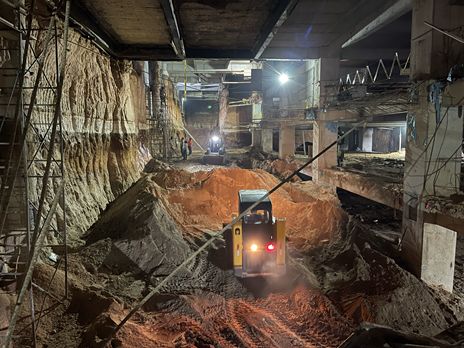
\includegraphics[width=0.65\linewidth]{imagenes_articulos/art02_01} \end{center}

\emph{Nota. }Elaboración propia. Fotografía tomada en el lugar del proyecto.

\end{minipage}
\end {flushleft}

El proyecto enfrentó también restricciones aéreas debido a su ubicación en la trayectoria de despegue del Aeropuerto Internacional La Aurora, lo cual limitó el uso de grúa torre hasta el nivel 8. Los niveles superiores fueron completados mediante sistemas de izaje manual con dispositivos de tracción mecánica, operados por cuadrillas especializadas en carga vertical. Un reto adicional fue la preservación de una ceiba (\emph{Ceiba pentandra}), árbol protegido por ley, que obligó a diseñar un sistema subterráneo de jardinería, de cuatro niveles, para mantener activas sus raíces durante y después del proceso constructivo.

\begin {flushleft}
\noindent\begin{minipage}[c]{\columnwidth}

\textbf{\figcaption{Área subterránea adaptada para preservar el sistema radicular de la ceiba}}

\begin{center}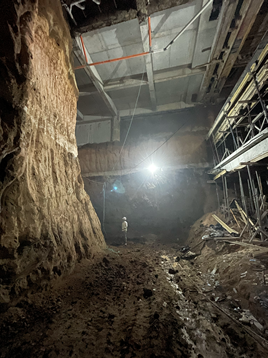
\includegraphics[width=0.65\linewidth]{imagenes_articulos/art02_02} \end{center}

\emph{Nota.} Elaboración propia. La fotografía corresponde al área en donde se preservó el sistema radicular de la ceiba.

\end{minipage}
\end {flushleft}

\hypertarget{justificaciuxf3n-del-muxe9todo-constructivo}{%
\subsection{Justificación del método constructivo}\label{justificaciuxf3n-del-muxe9todo-constructivo}}

Frente a las condiciones espaciales, ambientales y logísticas descritas, el método constructivo \emph{Top-Down} ofreció ventajas significativas frente al sistema tradicional \emph{Bottom-up}. Esta metodología permitió iniciar simultáneamente la construcción de la superestructura y la excavación descendente, redu-
ciendo el tiempo global de ejecución y limitando el impacto en la infraestructura vial y el entorno inmediato.

La losa de nivel calle funcionó como plataforma estructural de trabajo, brindando estabilidad temprana al perímetro del terreno y permitiendo la operación segura de maquinaria debajo de su superficie.

\hypertarget{secuencia-tuxe9cnica-aplicada}{%
\subsection{Secuencia técnica aplicada}\label{secuencia-tuxe9cnica-aplicada}}

El proceso constructivo inició con la perforación de pilotes \emph{in situ} como elementos de cimentación profunda. Posteriormente se fundió la losa a nivel de calle, que sirvió como base para las operaciones descendentes y ascendentes. Conforme se excavaban los niveles subterráneos se ejecutaban muros de pantalla para estabilizar el terreno. En paralelo, se avanzaba con la construcción de los niveles superiores, permitiendo el uso eficiente del tiempo y el espacio disponible.

\begin {flushleft}
\noindent\begin{minipage}[c]{\columnwidth}

\textbf{\figcaption{Fundición de muro pantalla mediante bombeo de concreto en nivel subterráneo}}

\begin{center}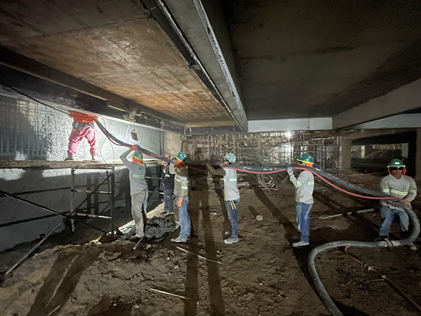
\includegraphics[width=0.8\linewidth]{imagenes_articulos/art02_03} \end{center}

\emph{Nota.} La fotografía corresponde al momento en que se fundió el muro de pantalla. Elaboración propia.

\end{minipage}
\end {flushleft}

\hypertarget{resultados-observados}{%
\subsection{Resultados observados}\label{resultados-observados}}

La implementación del método constructivo \emph{Top-Down} permitió la extracción controlada de aproximadamente 56,000 metros cúbicos de material, sin generar afectaciones sobre las vías circundantes ni interrumpir el tránsito urbano. Esta metodología facilitó la ejecución simultánea de cuatro niveles subterráneos y nueve niveles superiores, cumpliendo con el cronograma general del proyecto establecido entre julio de 2021 y diciembre de 2023.

\begin {flushleft}
\noindent\begin{minipage}[c]{\columnwidth}

\textbf{\figcaption{Vista final del edificio HUB Reforma}}

\begin{center}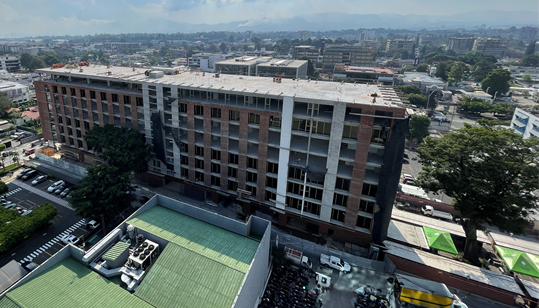
\includegraphics[width=1\linewidth]{imagenes_articulos/art02_04} \end{center}

\emph{Nota.} Elaboración propia. Visión panorámica del edificio Hub Reforma tras su ejecución con el sistema Top-Down.

\end{minipage}
\end {flushleft}

El sistema respondió de manera efectiva ante los principales desafíos del proyecto, incluyendo la geometría restringida del terreno, las restricciones impuestas por la franja aérea del Aeropuerto Internacional La Aurora, y la conservación de elementos naturales como la ceiba protegida. Estos resultados validan la eficiencia y adaptabilidad del sistema \emph{Top-Down} en contextos urbanos complejos, posicionándolo como una solución viable para proyectos de gran escala en ciudades con alta densidad.

\bigskip
\bigskip
\bigskip

\hypertarget{conclusiones-1}{%
\section{Conclusiones}\label{conclusiones-1}}

\begin{itemize}
\item
  La implementación del sistema \emph{Top-Down} en el edificio HUB Reforma permitió optimizar el tiempo de ejecución mediante la construcción simultánea de niveles subterráneos y superiores, garantizando la operatividad del entorno urbano durante todo el proceso.
\item
  El método demostró alta adaptabilidad frente a restricciones logísticas, geométricas y normativas, incluyendo la limitación aérea impuesta por el aeropuerto, la geometría reducida del terreno y la conservación de un árbol protegido dentro del volumen excavado.
\item
  La solución estructural basada en pilotes perforados \emph{in situ}, losa de arranque y muros pantalla proveyó estabilidad temprana al sistema y evidencia su viabilidad técnica para futuros proyectos en entornos urbanos densos de características similares.
\end{itemize}

\hypertarget{referencias-1}{%
\section{Referencias}\label{referencias-1}}

\begin{itemize}
\item
  {[}1{]} Barrientos, P. (2023). \emph{Cómo escribir un artículo con estilo APA: Pautas y consejos}. Acta Académica. \url{https://www.aacademica.org/pedro.barrientos/9.pdf}
\item
  {[}2{]} Geotech Rijeka. (2025). \emph{Top-down construction method}. \href{https://www.geotech.hr/en/top-down-construction-method/}{https://www.geotech.hr/en/top-down-
  construction-method/}
\item
  {[}3{]} Keller Cimentaciones. (2025). \emph{Muros pantalla}. \url{https://www.keller.com.es/experiencia/tecnicas/muros-pantalla}
\end{itemize}

\end {multicols}

\medskip

\HRule

\medskip

\hypertarget{art03}{%
\chapter{Diseño de la carretera interna y puente Badén en el CUNZAC: experiencia, resultados y aportes desde la Ingeniería Civil}\label{art03}}

\begin{center}
\includegraphics[width=1\linewidth]{autores/art03} \end{center}

\begin {multicols}{2}

\hypertarget{resumen-2}{%
\section{Resumen}\label{resumen-2}}

El presente articulo describe la experiencia adquirida durante el desarrollo del trabajo de graduación para obtener el título de ingeniero civil, en la modalidad de Ejercicio Profesional Supervisado. El proyecto consistió en el diseño de una carretera interna y un puente tipo badén para el Centro Universitario de Zacapa -CUNZAC- de la Universidad de San Carlos de Guatemala, con el objetivo de resolver uno de los problemas más críticos en el centro, el cual es la accesibilidad interna en el campus, agravándose este problema durante la época lluviosa, cuando el nivel del agua de la quebrada Carcal sube e interrumpe el paso peatonal y vehicular.

El proyecto desarrolló una fase de investigación y otra de servicio técnico profesional. En la fase de investigación, mediante el desarrollo del diagnóstico de inconformidades en el centro, se logró identificar la problemática de la accesibilidad y movilización interna; con base en esto se propuso el desarrollo de la carretera y un puente. En la fase técnica, se empezó con los estudios previos, los cuales abarcaron el levantamiento topográfico, análisis mecánico de suelos y estudio hidrológico. Con esta información se procedió con el diseño geométrico, hidráulico y estructural de la carretera y puente, lo cual resultó en una carretera de aproximadamente 1.5 km y puente badén de 47 metros de largo. En el transcurso de este proceso experimenté desafíos que fortalecieron mis capacidades técnicas y personales, adquiriendo una visión más realista de lo que implica el desarrollo de un proyecto de infraestructura civil y el impacto positivo que este genera en las comunidades más necesitadas.

El proyecto permitirá el acceso y movilidad interrumpida en el centro, beneficiando a más de 1,700 estudiantes del CUNZAC, así como a docentes, personal administrativo y futura comunidad universitaria creciente. Su implementación será un motor clave para el desarrollo integral y el crecimiento futuro no solo del centro universitario, sino también del municipio y departamento de Zacapa.

\hypertarget{abstract-2}{%
\section{Abstract}\label{abstract-2}}

This article describes the experience gained during the development of the graduation project to obtain the degree of Civil Engineer, under the modality of Supervised Professional Practice. The project consisted of the design of an internal road and a low-water bridge for the Zacapa University Center (CUNZAC) of the University of San Carlos of Guatemala, with the objective of solving one of the most critical problems at the center, which is internal accessibility within the campus. This problem worsens during the rainy season, when the water level of the Carcal stream rises and interrupts pedestrian and vehicular passage.

The project developed in two phases: an investigati-
ve phase and a professional technical service phase. In the investigative phase, through the diagnosis of problems at the center, the issue of internal accessibility and mobility was identified, based on which the development of the road and bridge was proposed. In the technical phase, preliminary studies were carried out, including topographic surveying, soil mechanical analysis, and hydrological study. With this information, the geometric, hydraulic, and structural design of the road and bridge was carried out. The result was a road approximately 1.5 km long and a 47-meter low-water bridge. Throughout this process, I experienced challenges that strengthened my technical and personal skills, acquiring a more realistic view of what the development of a civil infrastructure project entails and the positive impact it generates on the neediest communities.

The project will allow uninterrupted access and mobility within the center, benefiting more than 1,700 students of CUNZAC, as well as faculty, administrative staff, and the growing future university community. Its implementation will be a key driver for the comprehensive development and future growth not only of the university center but also of the municipality and department of Zacapa.

\hypertarget{palabras-claves-2}{%
\section{Palabras claves}\label{palabras-claves-2}}

Accesibilidad, infraestructura, educación, experien-
cia, Ingeniería.

\hypertarget{introducciuxf3n-2}{%
\section{Introducción}\label{introducciuxf3n-2}}

El Centro Universitario de Zacapa presenta una problemática importante de accesibilidad y movilización interna, la cual se agrava durante la época lluviosa, debido al aumento del nivel del agua en la quebrada Carcal. Esto ha dificultado el desarrollo y traslado total de sus actividades al campus propio, restringiendo el desarrollo académico y administrativo. De esta problemática surgió el proyecto de diseño de una carretera interna y un puente badén como solución. La experiencia adquirida durante este proceso me permitió aplicar conocimientos teóricos y prácticos en un contexto real, fortaleciendo mi formación profesional.

El objetivo de este artículo es compartir esa experiencia y resaltar el impacto positivo del proyecto, el cual permitirá mejorar las condiciones de acceso, facilitar el uso del terreno institucional y beneficiar directamente a la comunidad universitaria del CUNZAC. El trabajo representa una contribución concreta a la educación pública brindada por la Universidad de San Carlos de Guatemala.

\hypertarget{artuxedculo-1}{%
\section{Artículo}\label{artuxedculo-1}}

\hypertarget{contexto-y-justificaciuxf3n-del-proyecto}{%
\subsection{Contexto y justificación del proyecto}\label{contexto-y-justificaciuxf3n-del-proyecto}}

El Centro Universitario de Zacapa (CUNZAC) de la Universidad de San Carlos de Guatemala fue fundado en el año 2011; Inició labores en el año 2012 en las instalaciones del colegio Fredy Luna ubicado en la zona 1 de la ciudad de Zacapa. En la actualidad el centro universitario opera en las instalaciones del Colegio María Inmaculada, en las instalaciones del Colegio Nuestra Señora de Fátima, en la zona 1 del municipio de Zacapa y en un terreno propio de 15 manzanas, colindante a la aldea pueblo modelo.

El terreno de 15 manzanas se obtuvo gracias a un comité de profesionales en pro de la creación del centro universitario con instalaciones propias en Zacapa, donde realizaron varias gestiones para obtener un terreno adecuado para la construcción y traslado del centro universitario. Con la obtención del terreno, se empezaron a realizar las gestiones necesarias para empezar con el proceso de construc-
ción de los diferentes módulos de edificios que conformarán el centro universitario. En el año 2017 se inició la construcción de dos edificios, los cuales se finalizaron en el 2019, donde actualmente se encuentran construidos 4 edificios, conformando así los primeros dos módulos de edificios del centro universitario.

Al concluir la construcción de los edificios, estos se abrieron para iniciar las actividades académicas. A pesar de contar con ciertas instalaciones para el desarrollo de actividades específicas, se presenta un problema que frena el desarrollo de las actividades, ya que, durante la época lluviosa, el nivel del agua en la quebrada aumenta considerablemente, imposibilitando el acceso al campus. Además, la falta de una carretera interna resulta en caminos embarrados, lo que impide tanto el ingreso de vehículos como el tránsito seguro de estudiantes, profesores y personal administrativo.

Debido a este problema, dentro de la planificación conjunto del centro se decidió incorporar el diseño de una carretera interna y un puente tipo badén, que atravesara la quebrada permitiendo así el paso seguro de los vehículos. El desarrollo del proyecto se fundamenta en la importancia de garantizar un acceso seguro y confiable al campus durante todo el año. La falta de infraestructura vial en el campus obstaculiza el acceso continuo de los estudiantes, profesores y personal administrativo, y durante la época lluviosa lo imposibilita. Esta limitación no solo perjudica la asistencia a las clases, sino también al desarrollo de otras actividades académicas como prácticas, laboratorios, actividades extracurriculares, entre otras. Esto repercute directamente en el rendimiento académico, y la calidad de profesionales que egresan del CUNZAC.

Al realizar este proyecto, se establecerá una infraestructura sólida y resistente ante las inclemencias climáticas; la carretera y el puente tipo badén asegurarán que los estudiantes, profesores, personal administrativo y visitantes puedan movilizarse de manera segura y eficiente, generando así un entorno propicio para el desarrollo académico, laboral y social en el campus universitario. Al mejorar la conectividad y la accesibilidad, el proyecto contribuirá al crecimiento y desarrollo integral del Centro Universitario de Zacapa de la Universidad de San Carlos de Guatemala.

\hypertarget{experiencia-en-la-recopilaciuxf3n-de-datos}{%
\subsection{Experiencia en la recopilación de datos}\label{experiencia-en-la-recopilaciuxf3n-de-datos}}

Se recopilaron datos del sitio, y se efectuaron varias visitas técnicas; también hubo varias pláticas en relación con el proyecto, con el personal administrativo. Pudo evidenciarse la falta de una vía pavimentada, aunado a esto la presencia de la quebrada que atraviesa todo el terreno e interrumpe el paso hacia los módulos ya construidos. Es por ello que se propuso una vía pavimentada y un puente tipo badén para atravesar dicha quebrada en el punto más crítico.

Las visitas realizadas permitieron recopilar datos técnicos y sociales, como la población inscrita en el centro, la cantidad y tipos de vehículos en el día con mayor concurrencia, así como la topografía del lugar (incluyendo el cauce de la quebrada), la extracción de muestras de suelo específicas para la carretera y el puente, las cuales fueron analizadas en el laboratorio de mecánica de suelos de la Facultad de Ingeniería.

Las visitas al sitio fueron fundamentales para definir el trazo de la carretera, ubicar el puente y establecer parámetros reales de diseño. Además, representó un reto al organizar el trabajo en campo, validar información y adaptarse a las condiciones no controladas como el clima.

\hypertarget{estudios-tuxe9cnicos-realizados}{%
\subsection{Estudios técnicos realizados}\label{estudios-tuxe9cnicos-realizados}}

Para poder comenzar con el diseño del proyecto, se llevaron a cabo varios estudios. Se efectuó el estudio topográfico y se hizo un levantamiento topográfico del terreno, obteniendo la planimetría y altimetría del sitio. En específico se levantó el cauce de la quebrada para realizar posteriormente el estudio hidrológico, y así obtener los parámetros necesarios para los diseños hidráulicos del puente, así como los drenajes longitudinales y transversales).

\begin {flushleft}
\noindent\begin{minipage}[c]{\columnwidth}

\textbf{\figcaption{Vista 3D de la topografía del Centro Universitario de Zacapa Universidad de San Carlos de Guatemala}}

\begin{center}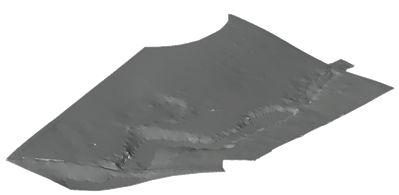
\includegraphics[width=1\linewidth]{imagenes_articulos/art03_01} \end{center}

\emph{Nota.} Elaboración propia.

\end{minipage}
\end {flushleft}

Con base en la topografía del cauce y la ubicación del campus se realizó el análisis hidrológico, identificando la microcuenca y obteniendo sus parámetros, para así obtener un caudal de diseño bajo un periodo de retorno de 100 años. Ya con en este caudal, se desarrollaron los diferentes diseños hidráulicos, como el drenaje transversal y longitudinal, y el de la tubería a colocar en el puente.

\begin {flushleft}
\noindent\begin{minipage}[c]{\columnwidth}

\textbf{\figcaption{Delimitación de la microcuenca, utilizada para determinar los parámetros hidrológicos del estudio}}

\begin{center}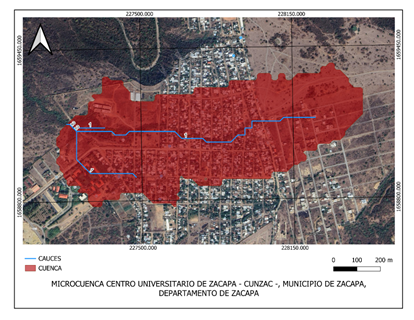
\includegraphics[width=1\linewidth]{imagenes_articulos/art03_02} \end{center}

\emph{Nota.} Elaboración propia, diseñado con QGISS Desktop 3.34.9.

\end{minipage}
\end {flushleft}

Tanto para el diseño de la carretera como para el diseño del puente, es necesario conocer la resistencia del suelo; para ello se extrajeron dos muestras; una que analizaría su resistencia a través del ensayo triaxial, obteniendo así los tres principales parámetros: la cohesión, densidad y el ángulo de fricción interna, para determinar la capacidad portante de suelo en el sitio donde se colocarán los estribos del puente. La otra muestra sirvió para determinar si el suelo natural es apto para utilizarse como subrasante en la carretera. Se trata del ensayo CBR (California Bearing Ratio). Con este resultado se pudo establecer si el suelo era apto para utilizarse como subrasante, y cuál podría ser el espesor de las capas del pavimento rígido.

\hypertarget{diseuxf1o-de-la-infraestructura}{%
\subsection{Diseño de la infraestructura}\label{diseuxf1o-de-la-infraestructura}}

Comenzando con la carretera, esta consiste en un circuito de aproximadamente 1.5 km, en el cual se incorporarán vías de retorno y una rotonda. El diseño geométrico de la carretera se basó en una carretera tipo D, según la clasificación por Tránsito Promedio Diario (TPD) de la Dirección General de Caminos (DGC). Para el diseño estructural del pavimento rígido se utilizó el método simplificado de la Portland Cement Association (PCA).

\begin {flushleft}
\noindent\begin{minipage}[c]{\columnwidth}

\textbf{\figcaption{Planta conjunto proyecto carretera interna}}

\begin{center}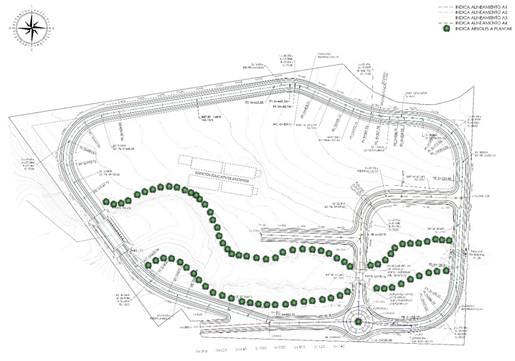
\includegraphics[width=0.95\linewidth]{imagenes_articulos/art03_03} \end{center}

\emph{Nota.} Elaboración propia, realizado con Autodesk Civil 3D 2025.

\end{minipage}
\end {flushleft}

Para el diseño de la rotonda del presente proyecto se tomaron en cuenta lo indicado en el Manual Centroamericano de Normas para el Diseño Geométri-
co de Carreteras y la Guía Informativa de Rotondas de la Administración Federal de Carreteras de Estados Unidos.

\begin {flushleft}
\noindent\begin{minipage}[c]{\columnwidth}

\textbf{\figcaption{Sección típica transversal del pavimento}}

\begin{center}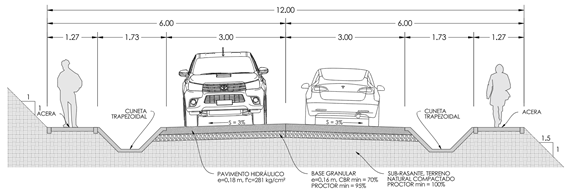
\includegraphics[width=0.95\linewidth]{imagenes_articulos/art03_04} \end{center}

\emph{Nota.} Elaboración propia, utilizando AutoCAD 2025.

\end{minipage}
\end {flushleft}

El segundo componente del proyecto es el diseño de un puente tipo badén con una longitud total de 47 metros, destinado a permitir el paso seguro sobre la quebrada Carcal. Esta quebrada presenta un cauce intermitente que se activa durante la época lluviosa, provocando la imposibilidad de acceder al campus desde el lado sur.

Para su diseño se realizó un estudio hidrológico e hidráulico utilizando el método racional con una intensidad de precipitación de 166.92 mm/h, un coeficiente de escorrentía de 0.80 y un tiempo de concentración de 17.24 minutos; se estimó un caudal máximo de diseño de 18.51 m³/s. Este representa las condiciones más críticas de crecida con un período de retorno de 100 años.

La solución hidráulica adoptada consistió en la colocación de once (11) tubos de concreto reforzado clase A de 48 pulgadas de diámetro, dispuestos de forma perpendicular al eje del puente. El dimensionamiento se realizó para asegurar que cada conducto opere a una fracción máxima de llenado del 75 \%, garantizando así su funcionamiento eficiente sin provocar desbordamientos.

La superestructura del puente está conformada por una losa de concreto hidráulico, de 16 cm de espesor, fundida sobre el concreto ciclópeo del cuerpo del puente y de los tubos. Sobre la banqueta y losa se construirán barandales de concreto armado, diseñados conforme a las especificaciones de la AASHTO LRFD Bridge Design Specifications (2020). El barandal fue diseñado para resistir cargas de impacto vehicular (nivel TL-3), sobrecarga peatonal y efectos de viento.

En cuanto a la subestructura, se diseñaron estribos de tipo muro de gravedad de concreto ciclópeo, con una altura de 4.00 metros y base de igual dimensión. Se realizaron verificaciones contra volteo, deslizamiento y capacidad de carga del suelo, aplicando factores de resistencia y diferentes combinaciones de carga. Finalmente se incorporaron aleros laterales, como guías de encauzamiento y una losa de concreto ciclópeo en la salida y entrada del flujo para evitar, socavación.

\begin {flushleft}
\noindent\begin{minipage}[c]{\columnwidth}

\textbf{\figcaption{Perfil del puente tipo badén}}

\begin{center}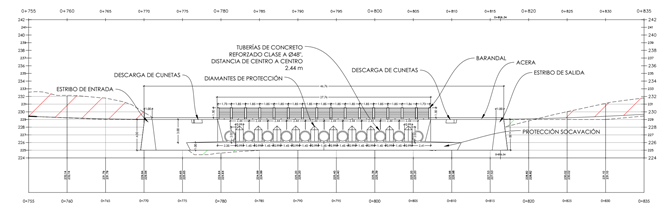
\includegraphics[width=0.95\linewidth]{imagenes_articulos/art03_05} \end{center}

\emph{Nota.} Elaboración propia, realizado con Autodesk Civil 3D 2025.

\end{minipage}
\end {flushleft}

El diseño se enfocó en brindar una solución resistente, de bajo costo y fácil mantenimiento, acorde con los recursos disponibles y el entorno físico del campus.

\hypertarget{aprendizaje-y-aporte-personal}{%
\subsection{Aprendizaje y aporte personal}\label{aprendizaje-y-aporte-personal}}

Este proyecto fue una de las experiencias más completas a lo largo de la etapa de estudiante. No solo se trató de aplicar conocimientos aprendidos en la carrera, sino también de enfrentar situaciones reales que exigieron criterio, análisis y bastante responsabilidad. Hubo aprendizaje para la toma de decisiones; se pudo organizar el trabajo en campo, utilizar nuevos programas, hacer planos constructivos, presupuestos y cronogramas; también revisar normas guatemaltecas e internacionales para avalar los diseños, y garantizar que estos sean seguros y funcionales.

Pero más allá de la parte técnica, este trabajo hizo ver el verdadero valor que tiene la ingeniería civil cuando se enfoca en resolver un problema o necesidad real. Saber que lo que uno diseña puede ayudar a una comunidad necesitada y resolver el problema por completo o coadyuvar en su minimización. La elaboración de este proyecto es una forma de devolverle algo a la Universidad de San Carlos de Guatemala. Todo lo aprendido durante estos años permitió llegar a este punto, y qué mejor manera de agradecerlo que aportando con una propuesta que beneficie directamente a una sede universitaria y a su comunidad, fortaleciendo uno de sus ejes estratégicos principales: la ``Extensión''.

\hypertarget{impacto-del-proyecto-y-beneficiarios}{%
\subsection{Impacto del proyecto y beneficiarios}\label{impacto-del-proyecto-y-beneficiarios}}

Este proyecto va a beneficiar directamente a más de 1,700 estudiantes que ya están inscritos en el CUNZAC, así como a los catedráticos y personal administrativo que allí labora. También facilitará que se puedan construir más aulas, laboratorios y otros espacios necesarios para que el CUNZAC pueda crecer, y brindar mejor educación, eliminando a la vez el costo de alquiler que se tiene actualmente. Este diseño no solo resuelve un problema puntual del acceso, sino que incentiva el desarrollo de toda la zona y fortalece la presencia de la USAC en el oriente del país. Es una inversión que va más allá de lo técnico, porque ayuda a que más personas tengan acceso a la educación superior, en un lugar con mejores condiciones.

\bigskip
\bigskip
\bigskip
\bigskip
\bigskip
\bigskip

\hypertarget{conclusiones-2}{%
\section{Conclusiones}\label{conclusiones-2}}

\begin{itemize}
\item
  Se diseñó y planificó la carretera interna y el puente badén para el Centro Universitario de Zacapa (CUNZAC), los cuales permitirán mejorar la accesibilidad, conectividad interna y seguridad para los estudiantes, docentes y personal administrativo, garantizando la operatividad durante todo el año, incluso en época lluviosa.
\item
  El desarrollo de este proyecto permitió aplicar de forma real todos los conocimientos aprendidos durante la carrera, y ayudó a entender mejor cómo funciona la ingeniería en situaciones reales.
\item
  Este trabajo representa un aporte a la USAC, ya que con este diseño se puede habilitar por completo el terreno del CUNZAC y mejorar la educación pública superior en la región.
\end{itemize}

\hypertarget{referencias-2}{%
\section{Referencias}\label{referencias-2}}

\begin{itemize}
\item
  {[}1{]} American Association of State Highway and Transportation Officials (2020). \emph{AASHTO LRFD Bridge Design Specifications}. (9th ed.). \href{https://aportesingecivil.com/aashto-lrfd-bridge-design-specifications-9th-edition-2020/}{https://aportesingecivil.com/aashto-lrfd-bridge-
  design-specifications-9th-edition-2020/}
\item
  {[}2{]} Dirección General De Caminos, Guatemala (2001). \emph{Especificaciones generales para la construc-
  ción de carreteras y puentes}. Editoriales Industriales.
\item
  {[}3{]} Federal Highway Administration (2000). \emph{Roundabouts: An Informational Guide} (FHWA-RD-
  00-067) \url{https://www.fhwa.dot.gov/publications/research/safety/00067/00067.pdf}
\item
  {[}4{]} Portland Cement Association (2020). \emph{Design of Concrete Pavement for City Streets}. \href{https://www.acpa.org/wpfd_file/design-of-concrete-pavement-for-streets-and-roads/}{https://www.
  acpa.org/wpfd\_file/design-of-concrete-pavement-
  for-streets-and-roads/}
\item
  {[}5{]} SIECA (2011). \emph{Manual de normas para el diseño geométrico de carreteras}. \href{https://www.sieca.int/producto/manual-de-normas-para-el-diseno-geometrico-de-carreteras/}{https://www.sieca.int/pro-
  ducto/manual-de-normas-para-el-diseno-geome-
  trico-de-carreteras/}
\end{itemize}

\end {multicols}

\medskip

\HRule

\medskip

\hypertarget{art04}{%
\chapter{Supervisión en campo, mi experiencia como epesista}\label{art04}}

\begin{center}
\includegraphics[width=1\linewidth]{autores/art04} \end{center}

\begin {multicols}{2}

\hypertarget{resumen-3}{%
\section{Resumen}\label{resumen-3}}

Durante mi EPS en la Regencia Norte de la Municipalidad de Guatemala, en el área de Obra Urbana, supervisé proyectos en ejecución en el Distrito 3 de la Zona 18. Me encargué de verificar avances físicos, el cumplimiento de planos y cronogramas, y asegurar la calidad de ejecución, lo que incluyó visitas constantes, elaboración de informes y comunicación directa con cuadrillas y vecinos. Uno de los momentos más impactantes fue presenciar en acción la maquina-
ria pesada, lo cual enriqueció mi comprensión respecto del proceso constructivo. Además, enfrenté desafíos técnicos innovadores y desarrollé habilidades en liderazgo empático y comunicación efectiva; de esa manera consolidé conocimientos teóricos y prácticos para mi desenvolvimiento profesional.

\hypertarget{abstract-3}{%
\section{Abstract}\label{abstract-3}}

During my EPS at the Regencia Norte of the Municipality of Guatemala, within the urban works department, I supervised projects in District 3 of Zone 18. My responsibilities included verifying progress, ensuring that blueprints and schedules were followed, and maintaining constant communication with work crews and residents. Moreover, witnessing heavy machinery in action and addressing innovative technical solutions greatly enhanced my leadership, empathy, and communication skills, marking a significant milestone in my professional development.

\hypertarget{palabras-claves-3}{%
\section{Palabras claves}\label{palabras-claves-3}}

Supervisión de obra, liderazgo empático, maquina-
ria, vecinos, metas.

\hypertarget{introducciuxf3n-3}{%
\section{Introducción}\label{introducciuxf3n-3}}

Desde el primer día, mi experiencia de realizar el EPS en la Regencia Norte de la Municipalidad de Guatemala se convirtió en la oportunidad perfecta para ver en acción lo que, a menudo, solo se estudia en teoría. Adentrarme en el Distrito 3 de la Zona 18, no solo me permitió supervisar proyectos en ejecución, sino también sumergirme en el dinamismo y los desafíos propios del trabajo en campo.

Este relato recoge el camino recorrido, en el que el control de avances, la verificación del cumplimiento de planos y cronogramas, y la supervisión del equipo humano se entrelazan para formar una experiencia inolvidable. Además, se destacan los aprendizajes diarios obtenidos a partir de la interacción directa con la maquinaria, los técnicos y, sobre todo, con la comunidad local, que transformó tanto la ciudad como mi formación profesional.

\hypertarget{artuxedculo-2}{%
\section{Artículo}\label{artuxedculo-2}}

Realicé mi EPS en la Regencia Norte de la Municipalidad de Guatemala, específicamente en el área de obra urbana. Aquí tuve la oportunidad y la responsabilidad de ejercer como supervisor de obra en algunos proyectos en ejecución en el Distrito 3 de la Zona 18 de la ciudad.

Esta experiencia permitió involucrarme de forma directa en el control y seguimiento de obras, verificando avances físicos, el cumplimiento de planos, cronogramas y la calidad de ejecución. Mi responsabilidad consistía en asegurarme de que cada proyecto se desarrollara conforme a lo planificado, lo cual implicaba visitas frecuentes al sitio, la elaboración de informes, la toma de evidencias fotográficas y, sobre todo, una constante interacción con las cuadrillas de trabajo y los vecinos del área.

Uno de los momentos que más me marcó fue ver por primera vez cómo opera la maquinaria en campo. En la universidad, muchas veces solo se ven imágenes o diagramas, pero presenciar en persona el funcionamiento real de equipos como retroexcavadoras, mezcladoras, bombas de concreto o camiones de volteo me permitió apreciar con mayor intensidad el trabajo que hay detrás de cada etapa constructiva.

\bigskip
\bigskip

También viví experiencias específicas que ampliaron mi visión como futuro profesional. Una de ellas fue la fundición de banquetas con concreto premezclado en callejones de difícil acceso. En este caso, el concreto fue bombeado a través de una tubería especial, ya que no era posible utilizar métodos convencionales. Esta solución técnica, pocas veces mencionada durante la carrera, me sorprendió por su ingenio y eficacia. Otro caso memorable fue la construcción de un parque en una zona que, anteriormente, estaba llena de maleza y en ocasiones se utilizaba como basurero. Semana a semana fui testigo de cómo el espacio se transformaba, dándole un nuevo sentido al área y beneficiando directamente a los vecinos; ver su felicidad al recibir un espacio limpio, verde y seguro fue profundamente gratificante.

\begin {flushleft}
\noindent\begin{minipage}[c]{\columnwidth}

\textbf{\figcaption{Parque construido}}

\begin{center}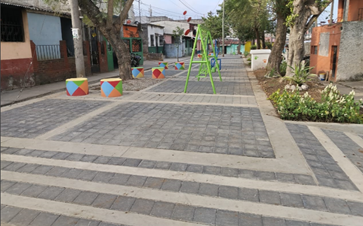
\includegraphics[width=0.8\linewidth]{imagenes_articulos/art04_01} \end{center}

\emph{Nota.} El parque fue construido en un área previamente degradada. Elaboración propia.

\end{minipage}
\end {flushleft}

\begin {flushleft}
\noindent\begin{minipage}[c]{\columnwidth}

\textbf{\figcaption{Banqueta de concreto premezclado fundida por medio de tubería}}

\begin{center}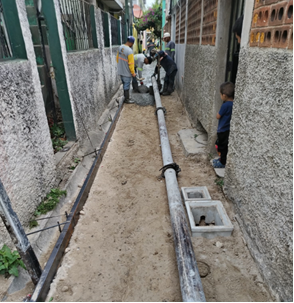
\includegraphics[width=0.8\linewidth]{imagenes_articulos/art04_02} \end{center}

\emph{Nota.} Fundición de banqueta en un callejón de difícil acceso. Elaboración propia.

\end{minipage}
\end {flushleft}

Además de lo aprendido en terreno, otro aspecto que valoro profundamente fue la calidad de las relaciones que logré construir dentro de la municipali-
dad. Desde los ingenieros y técnicos del área hasta los trabajadores de las cuadrillas, encontré personas dispuestas a compartir sus conocimientos, experiencias y formas de enfrentar los retos del día a día. Estas interacciones me enseñaron que el trabajo en equipo y el respeto mutuo son esenciales para que un proyecto avance de forma ordenada y eficiente. Aprendí a escuchar diferentes propuestas y experiencias, colaborar en la resolución de problemas y, sobre todo, a reconocer el valor de cada persona en la ejecución de una obra, sin importar su rol.

Durante mi tiempo como supervisor también reflexioné sobre el tipo de carácter que se necesita para liderar en campo. En mi caso, me considero una persona calmada y comprensiva, y procuré en todo momento ser empático con las situaciones personales y laborales de los trabajadores de cuadrilla, comprendiendo que cada uno enfrenta realidades distintas fuera del trabajo. Esta actitud me permitió generar confianza y mantener una comunicación abierta, facilitando un ambiente de colaboración y respeto mutuo. Sin embargo, también observé otros estilos de supervisión, más estrictos o autoritarios, donde se privilegia la disciplina por encima de la empatía. Si bien cada estilo tiene sus ventajas según el contexto, creo firmemente que un liderazgo basado en la comprensión y el respeto puede generar mejores resultados a largo plazo. Supervisar no es solo dirigir tareas; también implica saber escuchar, adaptarse y liderar con humanidad.

Ser epesista y, al mismo tiempo, ejercer funciones de supervisión fue un reto y a la vez una oportunidad única. Pude poner en práctica los conocimientos adquiridos en la universidad y desarrollar habilidades que difícilmente se enseñan en el aula: liderazgo, comunicación efectiva, adaptación al cambio y gestión del tiempo. Esta etapa marcó un antes y un después en mi formación profesional.

\hypertarget{conclusiones-3}{%
\section{Conclusiones}\label{conclusiones-3}}

\begin{itemize}
\item
  Mi experiencia durante el periodo que duró el EPS me permitió consolidar lo aprendido en la universidad y aplicarlo en el campo, desarrollando habilidades técnicas como el control y seguimiento de obras, destrezas prácticas en la supervisión de maquinaria y manejo de desafíos de ejecución. Esta etapa evidenció que, para alcanzar buenos resultados en proyectos de obra urbana, es fundamental una combinación equilibrada de conocimientos teóricos y habilidades prácticas, permitiéndome enfrentar de manera efectiva los retos del terreno.
\item
  La interacción constante con ingenieros, técnicos, cuadrillas y la comunidad, reforzó la idea de que el liderazgo en campo va más allá de la simple dirección de tareas; implica una comunicación abierta, empatía y la capacidad de adaptar el estilo de supervisión a las necesidades reales del equipo y del proyecto. Este enfoque no solo favoreció el cumplimiento de los objetivos técnicos, sino que también propició un ambiente de colaboración y respeto, marcando un hito significativo en mi crecimiento profesional y personal.
\end{itemize}

\hypertarget{referencia}{%
\section{Referencia}\label{referencia}}

\begin{itemize}
\tightlist
\item
  {[}1{]} Forbes Argentina. (2022, 27 abril). \emph{Qué es el ``liderazgo empático'' y cuáles son sus beneficios}. \href{https://www.forbesargentina.com/liderazgo/que-liderazgo-empatico-cuales-son-sus-beneficios-n15335}{https://www.forbesargentina.com/liderazgo/que-
  liderazgo-empatico-cuales-son-sus-beneficios-
  n15335}
\end{itemize}

\end {multicols}

\medskip

\HRule

\medskip

\hypertarget{art05}{%
\chapter{Diseño del proceso de dotación de talento humano en GAIA Business School, Guatemala}\label{art05}}

\begin{center}
\includegraphics[width=1\linewidth]{autores/art05} \end{center}

\begin {multicols}{2}

\hypertarget{resumen-4}{%
\section{Resumen}\label{resumen-4}}

El presente proyecto, dividido en tres fases, aborda el diseño de un proceso sólido de dotación de talento humano, entendido como el conjunto de pasos necesarios para encontrar y contratar a las personas adecuadas para un puesto específico. El proceso desarrollado permite identificar y controlar de manera significativa el porcentaje de rotación, uno de los principales problemas organizacionales. Esto ha fortalecido a la empresa, ya que contar con el talento calificado le permite ejecutar sus operaciones de manera exitosa.

El proceso inicia con una planificación estratégica y continúa con las etapas de búsqueda, selección, contratación, inducción, desarrollo profesional, transferencia, desvinculación laboral y mejora continua, consolidando así un ciclo completo de gestión de talento. Para su implementación se elaboraron manuales, guías y formatos que orientan al responsable de cada etapa. Además, se documentaron descriptores y perfiles de puesto para que los colaboradores comprendan claramente sus funciones y responsabilidades. Como parte del compromiso con la sostenibilidad, se diseñó un plan de concientización sobre el ahorro de papel en las oficinas, contribuyendo al cuidado del medio ambiente y a la reducción de costos operativos. Finalmente, se desarrolló un plan anual de capacitación, con el objetivo de fomentar el crecimiento continuo de los colaboradores.

\hypertarget{abstract-4}{%
\section{Abstract}\label{abstract-4}}

This Project, structured in three phases, focuses on the design of a robust human talent staffing process, understood as the series of steps necessary to find and hire the right individuals for specific positions. The developed process enables the organization to significantly identify and control employee turnover, one of the main organizational challenges. This has strengthened the company, as having qualified talent allows it to carry out its operations successfully. The process begins with strategic planning and continues through the stages of recruitment, selection, hiring, Onboarding, profesional development, internal transfers, offboarding, and continuous improvement, thus consolidating a complete talent management cycle. For its implementation, manuals, guidelines, and templates were developed to guide those responsible for each stage. Additionally, job descriptors and profiles were documented to ensure that employees crearly understand their roles and responsibilities. As part of the organization´s commit-
ment to sustainability, a paper-saving awareness plan was designed for office use, contributing to environmental protection and reducing operational costs. Finally, an annual training plan was created to promote the continuous professional development of employees.

\hypertarget{palabras-claves-4}{%
\section{Palabras claves}\label{palabras-claves-4}}

Contratación, rotación laboral, capacitación, recursos humanos, reclutamiento, selección.

\hypertarget{introducciuxf3n-4}{%
\section{Introducción}\label{introducciuxf3n-4}}

La gestión del talento humano ha dejado de ser una función meramente operativa para convertirse en un eje estratégico dentro de las organizaciones modernas. Uno de los problemas más frecuentes que enfrentan las empresas es la alta rotación laboral, la cual afecta negativamente la productividad, incrementa los costos y debilita la estabilidad de los equipos de trabajo (Chiavenato, 2011). En este contexto, contar con un proceso estructurado de dotación de talento humano permite atraer, seleccionar y retener al talento adecuado para cada puesto. Tal como señala Alles (2019), una gestión basada en competencias aporta claridad y coherencia en cada etapa del ciclo de vida del colaborador. Por su parte, Dessler (2009) destaca la importancia de diseñar políticas y prácticas que acompañen el desarrollo continuo del recurso humano. Este proyecto busca responder a estas necesidades mediante un modelo integral y sostenible que fortalezca el capital humano y aporte valor real a la organización.

\hypertarget{artuxedculo-3}{%
\section{Artículo}\label{artuxedculo-3}}

\hypertarget{diagnuxf3stico}{%
\subsection{Diagnóstico}\label{diagnuxf3stico}}

Como punto de partida para este proyecto se realizó un diagnóstico mediante un diagrama de Ishikawa, el cual identificó como problema principal la inadecuada gestión del talento humano en la empresa. A través del análisis de las causas distribuidas en las categorías de las 6M (método, mano de obra, materiales, maquinaria, medición y medio ambiente), se evidenció que la falta de procedimientos claros, la ausencia de planificación, y la contratación de personal sin el perfil adecuado afectan directamente al desempeño organizacional. El efecto más relevante identificado fue una alta rotación de personal, alimentada por la integración deficiente del nuevo talento por falta de inducción. Como causa raíz, se determinó un proceso de selección inadecuado, ya que contratar a personas sin las competencias requeridas genera insatisfacción y desvinculación temprana.

\hypertarget{proceso-de-dotaciuxf3n-de-talento-humano}{%
\subsection{Proceso de dotación de talento humano}\label{proceso-de-dotaciuxf3n-de-talento-humano}}

El proceso de dotación de talento humano es un conjunto ordenado de etapas que permiten a una organización atraer, seleccionar, integrar, desarrollar y, en caso necesario, desvincular al personal de forma estratégica. Este proceso fue diseñado con base en las necesidades identificadas durante el diagnóstico organizacional, y está representado mediante un diagrama de bloques que ilustra el flujo lógico de cada fase tal como se muestra en la siguiente figura.

\begin {flushleft}
\noindent\begin{minipage}[c]{\columnwidth}

\textbf{\figcaption{Diagrama de bloques que muestra cada fase del proceso de dotación de talento humano}}

\begin{center}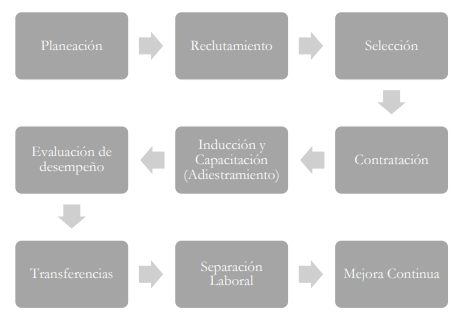
\includegraphics[width=0.95\linewidth]{imagenes_articulos/art05_01} \end{center}

\emph{Nota.} Elaboración propia, utilizando software Microsoft Visio.

\end{minipage}
\end {flushleft}

A continuación, se describen las etapas que conforman este proceso; cabe resaltar que, para realizar esta gestión de manera precisa y eficiente, el encargado de cada gestión puede apoyarse en guías, manuales y formatos diseñados para trazar el camino y cumplir con todos los requerimientos:

\begin{itemize}
\item
  Planeación: en esta fase se identifican las necesidades de personal con base en los objetivos estratégicos de la empresa. Se analizan vacantes, cargas de trabajo y competencias requeridas para anticipar futuras contrataciones; para realizar esto son de mucha ayuda los descriptores y perfiles de puesto.
\item
  Reclutamiento: consiste en atraer candidatos potenciales a través de fuentes internas y externas. Se definen los canales de difusión, los requisitos del puesto y los criterios de preselección.
\item
  Selección: se evalúan los perfiles de los candidatos mediante entrevistas, pruebas psicométricas y técnicas, verificaciones de referencias y filtros alineados al perfil de puesto previamente diseñado.
\item
  Contratación: una vez seleccionado el candidato adecuado, se formaliza su ingreso a través de un contrato, cumpliendo con los requisitos legales y administrativos correspondientes.
\item
  Inducción y capacitación: en esta etapa se brinda al nuevo colaborador la información necesaria sobre la empresa, su cultura, políticas y funciones específicas. Se facilita también la capacitación inicial para el desempeño eficiente de sus tareas.
\item
  Evaluación de desempeño: se monitorea el rendimiento del colaborador en función de metas y competencias definidas. Se ha implementado la evaluación 360 grados para abarcar mejor el rendimiento del colaborador. Esta etapa permite identificar fortalezas, áreas de mejora y oportunidades de desarrollo.
\item
  Transferencias: permite la reubicación interna del personal en función a sus habilidades, intereses y las necesidades de la empresa; se han implementado tres tipos, la transferencia vertical, horizontal y diagonal, promoviendo la retención y el crecimiento profesional.
\item
  Separación laboral: se gestiona de forma ordenada y respetuosa la desvinculación de un colaborador, ya sea por renuncia, terminación de contrato o jubilación. Se documenta el proceso para fines administrativos y de mejora.
\item
  Mejora continua: se realiza una revisión periódica del proceso en su totalidad para identificar oportunidades de optimización, incorporando retroalimentación, indicadores de desempeño, y tendencial del entorno; para esta etapa se utilizó el ciclo de Deming o ciclo PDCA.
\end{itemize}

\hypertarget{caracteruxedsticas-del-proceso-de-dotaciuxf3n-de-talento-humano}{%
\subsection{Características del proceso de dotación de talento humano}\label{caracteruxedsticas-del-proceso-de-dotaciuxf3n-de-talento-humano}}

\begin{itemize}
\item
  Sistematización: el proceso sigue una secuencia lógica de etapas definidas, lo cual facilita su ejecución de forma ordenada y consistente, evitando improvisaciones y garantizando unifor-
  midad en la gestión.
\item
  Trazabilidad: cada etapa deja evidencia documen-
  tal que permite verificar decisiones tomadas, analizar indicadores de eficiencia y generar mejoras a partir de datos objetivos.
\item
  Adaptabilidad: el proceso diseñado puede ajustarse a distintos contextos y necesidades organizacionales, manteniendo su estructura general, pero permitiendo adaptaciones según el tamaño o naturaleza de la empresa.
\end{itemize}

\hypertarget{ventajas-de-contar-con-un-diseuxf1o-suxf3lido-de-dotaciuxf3n-de-talento-humano}{%
\subsection{Ventajas de contar con un diseño sólido de dotación de talento humano}\label{ventajas-de-contar-con-un-diseuxf1o-suxf3lido-de-dotaciuxf3n-de-talento-humano}}

\begin{itemize}
\item
  Mejora en la calidad del talento incorporado: un proceso bien estructurado permite definir con precisión los perfiles requeridos y aplicar filtros adecuados durante la selección. Esto asegura que los candidatos contratados posean las competencias técnicas y actitudinales necesarias al puesto.
\item
  Reducción de la rotación de personal: al contratar personal alineado con el perfil del puesto y brindarles una adecuada inducción y seguimiento, se incrementa la satisfacción laboral, lo cual disminuye la rotación y sus costos asociados.
\item
  Optimización de los costos de contratación: la planificación y estandarización del proceso reducen gastos innecesarios derivados de errores en la contratación, repeticiones de procesos o tiempos prolongados de vacantes sin cubrir.
\end{itemize}

\hypertarget{diagrama-de-reclutamiento-y-selecciuxf3n}{%
\subsection{Diagrama de reclutamiento y selección}\label{diagrama-de-reclutamiento-y-selecciuxf3n}}

A continuación, se presenta el diagrama de flujo de reclutamiento y selección que se considera el corazón de todo el proceso, debido a que depende de estos si el colaborador se apega a todos los requerimientos del puesto y asegura su permanencia en la empresa.

\begin {flushleft}
\noindent\begin{minipage}[c]{\columnwidth}

\textbf{\figcaption{Diagrama de flujo del procedimiento de reclutamiento de personal}}

\begin{center}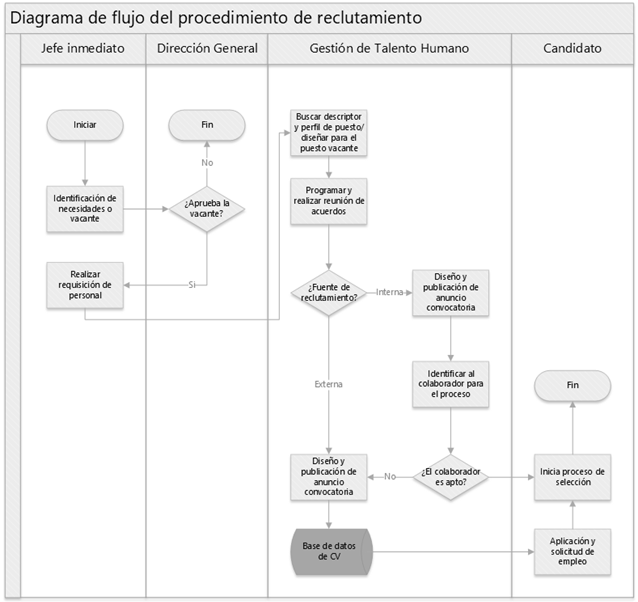
\includegraphics[width=0.8\linewidth]{imagenes_articulos/art05_02} \end{center}

\emph{Nota.} Elaboración propia, utilizando software Microsoft Visio.

\end{minipage}
\end {flushleft}

\begin {flushleft}
\noindent\begin{minipage}[c]{\columnwidth}

\textbf{\figcaption{Diagrama de flujo del procedimiento de selección de personal}}

\begin{center}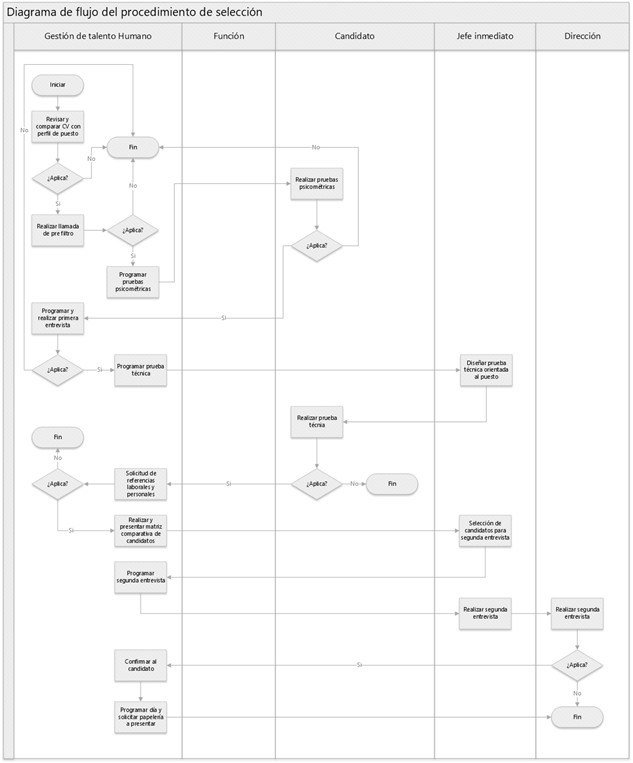
\includegraphics[width=0.8\linewidth]{imagenes_articulos/art05_03} \end{center}

\emph{Nota.} Elaboración propia, utilizando software Microsoft Visio.

\end{minipage}
\end {flushleft}

\hypertarget{conclusiones-4}{%
\section{Conclusiones}\label{conclusiones-4}}

\begin{itemize}
\item
  Un proceso sólido y bien estructurado de dotación de talento humano no solo contribuye a la reducción de la rotación de personal, sino que también fortalece la capacidad de la organización para alcanzar sus objetivos estratégicos. La planificación, selección adecuada y desarrollo profesional continuo son pilares fundamentales para el éxito organizacional.
\item
  La implementación de herramientas y metodolo-
  gías, como manuales y perfiles de puesto, garantiza que cada etapa del proceso sea consistente, medible y adaptable. Esto permite optimizar recursos y tomar decisiones informadas basadas en indicadores de desempeño.
\item
  Al incorporar talento adecuado y fomentar su desarrollo profesional, el proceso de dotación genera un ambiente laboral más estable, motivador y colaborativo. Además, iniciativas complementarias como la concientización ambiental benefician tanto a la empresa como al medio ambiente, promoviendo una gestión responsable.
\end{itemize}

\hypertarget{recomendaciones}{%
\section{Recomendaciones}\label{recomendaciones}}

\begin{itemize}
\item
  Establecer mecanismos de seguimiento para asegurar que el plan de capacitación anual responda a las necesidades emergentes de la organización y a los cambios en el entorno. Esto incrementará la competitividad del talento y su compromiso con la empresa.
\item
  Monitorear y evaluar el desempeño del proceso de dotación mediante indicadores clave como tiempo de contratación, porcentaje de rotación y satisfacción del personal. Usar los resultados para ajustar y mejorar continuamente cada etapa.
\end{itemize}

\bigskip
\bigskip
\bigskip
\bigskip
\bigskip
\bigskip

\begin{itemize}
\tightlist
\item
  Integrar soluciones basadas en IA no solo puede optimizar significativamente diversas etapas del proceso, como la revisión de currículums, análisis de competencias, predicción de rotación o desempeño, y automatización del seguimiento a candidatos para agilizar la toma de decisiones, sino que también mejora la precisión en la selección de talento totalmente alineado al perfil requerido, fortaleciendo la efectividad del proceso.
\end{itemize}

\hypertarget{referencias-3}{%
\section{Referencias}\label{referencias-3}}

\begin{itemize}
\item
  {[}1{]} Alles, M. (2005). \emph{Gestión del talento humano basado en competencias}. Editorial Granica. \href{https://drive.google.com/file/d/1o-kqZKqmhSITxWv-QIM_BN7j5LkJ3UaH/view}{https://drive.google.com/file/d/1o-kqZKqmhSITx
  Wv-QIM\_BN7j5LkJ3UaH/view}
\item
  {[}2{]} Alles, M. (2006). \emph{Dirección estratégica de recursos humanos}. Editorial Granica. \href{https://www.bqm.com.pe/libros/Martha\%20Alles\%20-\%20Direccion\%20estrategica\%20de\%20recursos\%20humanos\%20-\%20Casos.pdf}{https://www.
  bqm.com.pe/libros/Martha Alles - Direccion estrategica de recursos humanos - Casos.pdf}
\item
  {[}3{]} Chiavenato, I. (2015). \emph{Gestión del talento humano}. McGraw-Hill. \url{https://archive.org/details/gestion-del-talento-humano-3e}
\item
  {[}4{]} Dessler, G. (2001). \emph{Administración de personal}. Pearson. \href{https://universitad.com/economia-y-finanzas/administracion-de-personal-6-edicion-gary-dessler/}{https://universitad.com/economia-y-fi-
  nanzas/administracion-de-personal-6-edicion-ga-
  ry-dessler/}
\item
  {[}5{]} Dessler, G. (2009). \emph{Administración de recursos humanos}. Pearson Educación. \href{https://studylib.es/doc/8849041/administracion-de-recursos-humanos-11va-dessler-1?p=3}{https://studylib.es/
  doc/8849041/administracion-de-recursos-huma
  nos-11va-dessler-1?p=3}
\item
  {[}6{]} Ivancevich, J. (2005). \emph{Administración de recursos humanos}. McGraw-Hill. \href{https://es.scribd.com/document/358298940/Ivancevich-2005-Administracion-de-RH-8-Seleccion-de-Recursos-Humanos}{https://es.scribd.
  com/document/358298940/Ivancevich-2005-Ad-
  ministracion-de-RH-8-Seleccion-de-Recursos-Hu-
  manos}
\end{itemize}

\end {multicols}

\medskip

\HRule

\medskip

\hypertarget{art06}{%
\chapter{Evaluación de aguas residuales domésticas provenientes de una planta de tratamiento ubicada en la residencial San Ángel 4, zona 2, por medio del índice simplificado de calidad del agua (ISQA)}\label{art06}}

\begin{center}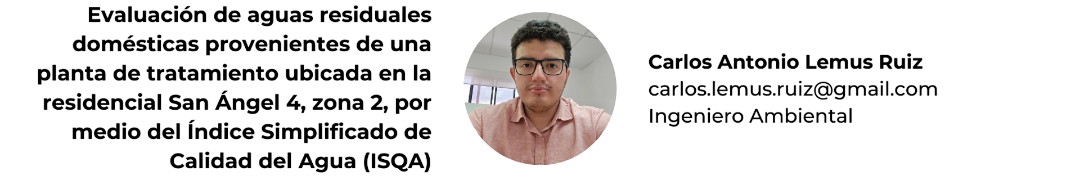
\includegraphics[width=1\linewidth]{autores/art06} \end{center}

\begin {multicols}{2}

\hypertarget{resumen-5}{%
\section{Resumen}\label{resumen-5}}

Se evaluó la eficacia de una planta de tratamiento durante la época lluviosa y seca, comparando los valores medios de los puntos de muestreo con los límites máximos permisibles (LMP), a partir de un conjunto de parámetros regulados en el AG 236-2006 y que permiten realizar una clasificación en el ISQA.

Con apoyo del Laboratorio ECOQUIMSA se recolectó un total de 12 muestras entre ambas épocas, siendo los puntos de muestreo el afluente previo al ingreso a la planta de tratamiento y el efluente de descarga, que posteriormente analizaron en sus instalaciones.

Los resultados indican que los parámetros se encuentran dentro de los LMP, exceptuando ``grasas y aceites'' y ``coliformes fecales'' en ambas épocas, pero durante la época seca la ``DBO5'' supera el LMP. En las épocas en mención existe una eficacia de remoción positiva en la mayoría de los parámetros, y destaca una eficacia mayor a 95 \% en la remoción de ``coliformes fecales'', pero en la época seca la eficacia de remoción es negativa para ``Nitrógeno total'' y ``color'', indicando que el valor de estos parámetros aumenta al pasar por la planta de tratamiento. Respecto del ISQA, en ambas épocas existe una diferencia mínima entre la entrada y salida, siendo clasificados como ``Inadmisibles'', dando a entender que la calidad del agua continúa siendo inferior y disminuye la posibilidad de encontrar un uso para el cuerpo receptor.

\hypertarget{abstract-5}{%
\section{Abstract}\label{abstract-5}}

The efficiency of a treatment plant was evaluated during both the rainy and dry seasons by comparing the average values of sampling points with the Maximum Permissible Limits (MPL), based on a set of parameters regulated by AG 236-2006, which also allow for classification under the ISQA.

With support from the ECOQUIMSA Laboratory, a total of 12 samples were collected across both seasons. The sampling points were the influent (prior to entering the treatment plant) and the effluent (discharge point), which were subsequently analyzed at the laboratory's facilities.

The results indicate that the parameters were within the MPL, with the exception of ``Fats and Oils'' and ``Fecal Coliforms'' in both seasons. However, during the dry season, ``BOD₅'' exceeded the MPL. In both seasons, there was a positive removal efficiency for most parameters, with removal of ``Fecal Coliforms'' standing out at over 95\%. Nevertheless, during the dry season, the removal efficiency was negative for ``Total Nitrogen'' and ``Color'', indicating that the values of these parameters increased after passing through the treatment plant.

Regarding the ISQA, in both seasons there was minimal difference between influent and effluent values, and the water was classified as ``Unacceptable'', suggesting that the water quality remains poor and reduces the likelihood of any beneficial use for the receiving body.

\hypertarget{palabras-claves-5}{%
\section{Palabras claves}\label{palabras-claves-5}}

Aguas residuales, AG 236-2006, ISQA, LMP.

\hypertarget{introducciuxf3n-5}{%
\section{Introducción}\label{introducciuxf3n-5}}

El tratamiento de las aguas residuales permite reducir la carga de contaminación que reciben los cuerpos receptores en Guatemala a diario. Las diferentes instalaciones encargadas de este tratamiento requieren un monitoreo anual para controlar su eficacia al momento de regular diferentes parámetros físicos, químicos y biológicos presentes en las aguas residuales. El Acuerdo Gubernativo 236-2006 ``Reglamento de las descargas y reuso de aguas residuales y la disposición de lodos'', estipula los límites máximos permisibles de parámetros regulados que deben cumplir los entes generadores.
En la Región Metropolitana de Guatemala, hay aproximadamente 1066 plantas de tratamiento, de las cuales la mayoría en caso de funcionar, lo hace deficientemente y sin cumplir la normativa de descarga establecida. Además, existen 2700 entes generadores de aguas residuales que descargan su efluente sin mayor monitoreo ni control por las autoridades correspondientes (Funcagua, 2022).

\hypertarget{artuxedculo-4}{%
\section{Artículo}\label{artuxedculo-4}}

\hypertarget{objetivo}{%
\subsection{Objetivo}\label{objetivo}}

Se realizó una caracterización de las aguas residuales de origen doméstico provenientes de una residencial ubicada en la ciudad de Guatemala para comparar con los límites máximos permisibles de los parámetros regulados en el AG 236-2006 y determinar la eficacia del sistema de tratamiento que emplean en época lluviosa y época seca. Utilizando el Índice Simplificado de Calidad del Agua (ISQA) se calculó su valor y se clasificó tanto el afluente como el efluente de las instalaciones de tratamiento, para posteriormente comparar.

\hypertarget{metodologuxeda}{%
\subsection{Metodología}\label{metodologuxeda}}

Se basó en un enfoque cuantitativo del análisis de la calidad del agua y parámetros de estudio establecidos en el artículo 24 del AG 236-2006, orientados en aguas residuales de origen doméstico sin tomar en cuenta los relacionados a metales pesados, adicionando los parámetros requeridos para el cálculo del ISQA y su respectiva clasificación. La recolección de muestras se llevó a cabo en un punto previo al ingreso de las aguas residuales a la planta de tratamiento y en un punto en la descarga (2 puntos de muestreo en total), realizado tanto en la época lluviosa como en la época seca. Se efectuaron 3 repeticiones para cada punto de muestreo y en cada época, dando un total de 12 muestras recolectadas (6 por cada época). La planta de tratamiento pertenece a Residencial San Ángel 4, y está ubicada en los límites de la zona 2 de la ciudad de Guatemala que colindan con los de Chinautla.

\hypertarget{resultados}{%
\subsection{Resultados}\label{resultados}}

Con base en los parámetros del Acuerdo Gubernativo 236-2006, la planta de tratamiento de agua residual en estudio se encuentra ubicada en una zona residencial; en consecuencia, las aguas residuales domésticas no contienen metales pesados y por tal razón los parámetros del Acuerdo Gubernativo 236-2006 que son muestreados y estudiados son: temperatura, pH, grasas y aceites, materia flotante, sólidos suspendidos totales, DBO5, DQO, nitrógeno total, fósforo total, color y coliformes fecales. Para el cálculo del ISQA los parámetros muestreados y estudiados son temperatura, DQO, sólidos suspendidos totales, conductividad eléctrica y oxígeno disuelto.

\begin {flushleft}
\noindent\begin{minipage}[c]{\columnwidth}

\textbf{\tabcaption{Eficacia de la planta de tratamiento en épocas de estudio}}

\begin{center}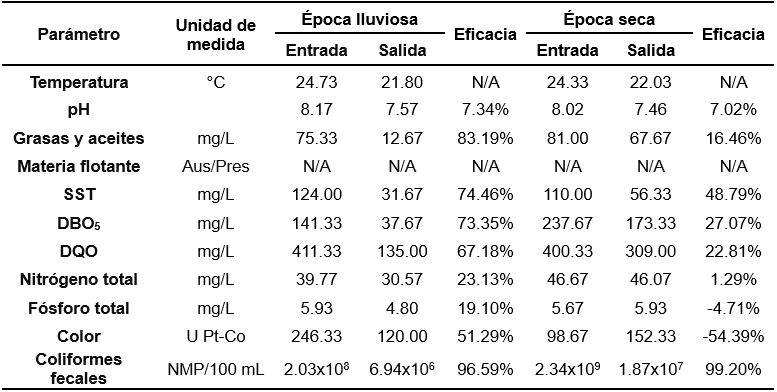
\includegraphics[width=1\linewidth]{imagenes_articulos/art06_01} \end{center}

\emph{Nota.} Elaboración propia.

\end{minipage}
\end {flushleft}

\begin {flushleft}
\noindent\begin{minipage}[c]{\columnwidth}

\textbf{\figcaption{Gráfica de comparación de la eficacia entre las épocas de estudio}}

\begin{center}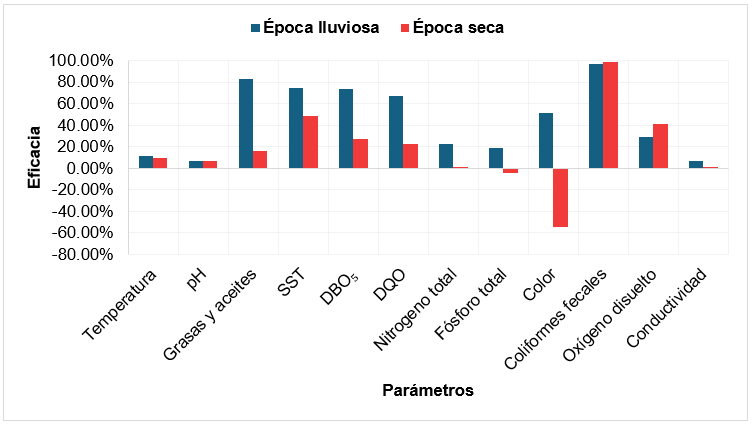
\includegraphics[width=1\linewidth]{imagenes_articulos/art06_02} \end{center}

\emph{Nota.} Elaboración propia.

\end{minipage}
\end {flushleft}

\begin {flushleft}
\noindent\begin{minipage}[c]{\columnwidth}

\textbf{\tabcaption{Cumplimiento de parámetros para etapa II del AG 236-2006 durante épocas de estudio}}

\begin{center}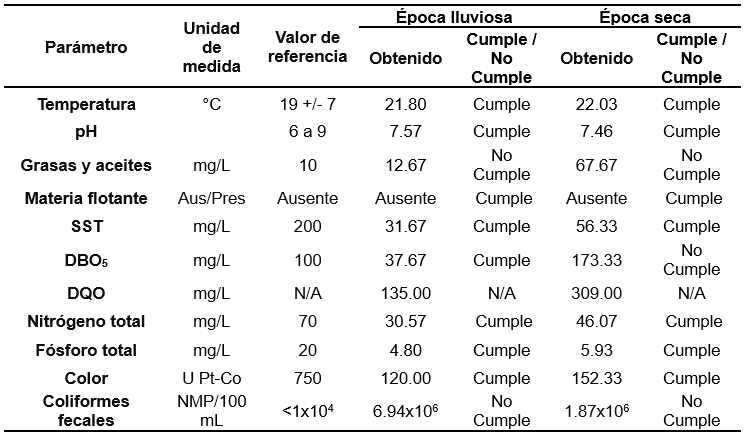
\includegraphics[width=1\linewidth]{imagenes_articulos/art06_03} \end{center}

\emph{Nota.} Elaboración propia.

\end{minipage}
\end {flushleft}

\begin {flushleft}
\noindent\begin{minipage}[c]{\columnwidth}

\textbf{\tabcaption{Clasificación de la calidad de agua del ISQA}}

\begin{center}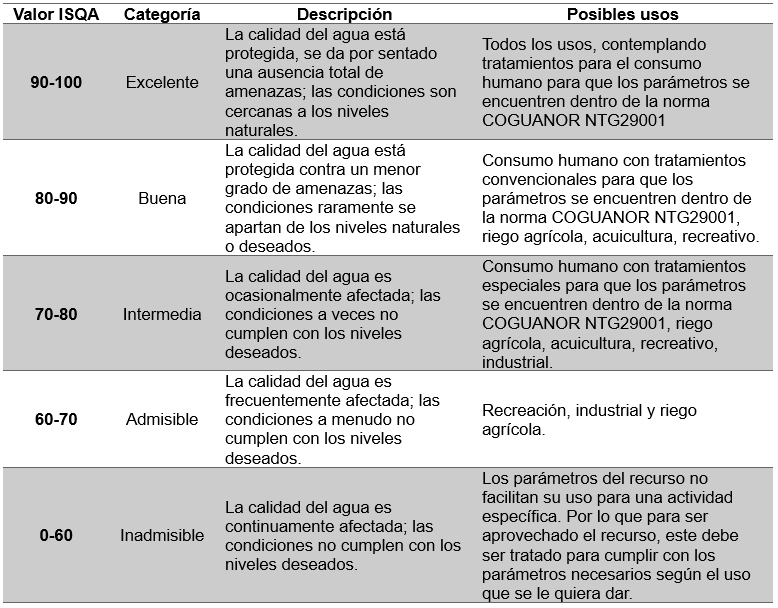
\includegraphics[width=1\linewidth]{imagenes_articulos/art06_04} \end{center}

\emph{Nota.} INSIVUMEH, 2021.

\end{minipage}
\end {flushleft}

\begin {flushleft}
\noindent\begin{minipage}[c]{\columnwidth}

\textbf{\tabcaption{Valores calculados del ISQA para épocas de estudio}}

\begin{center}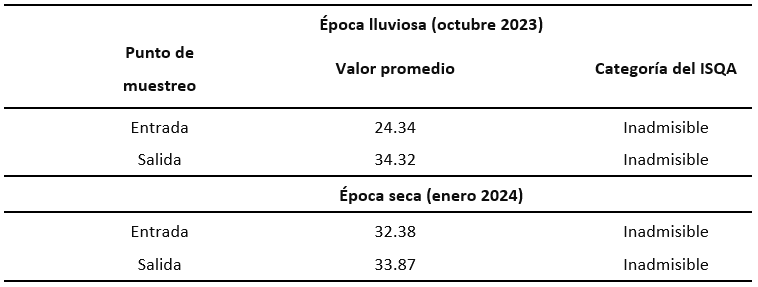
\includegraphics[width=1\linewidth]{imagenes_articulos/art06_05} \end{center}

\emph{Nota.} Elaboración propia.

\end{minipage}
\end {flushleft}

\begin {flushleft}
\noindent\begin{minipage}[c]{\columnwidth}

\textbf{\figcaption{Gráfica de comparación del ISQA promedio en épocas de estudio}}

\begin{center}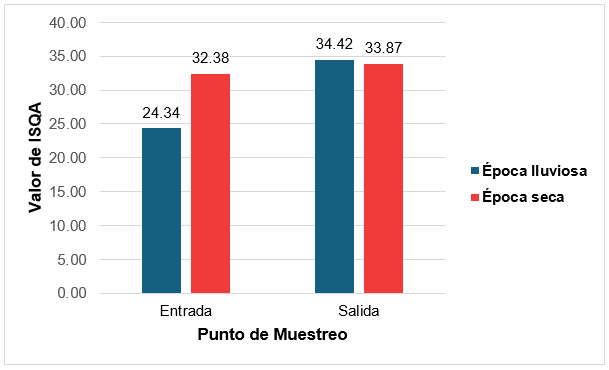
\includegraphics[width=1\linewidth]{imagenes_articulos/art06_06} \end{center}

\emph{Nota.} Elaboración propia.

\end{minipage}
\end {flushleft}

\bigskip
\bigskip
\bigskip
\bigskip
\bigskip
\bigskip

\hypertarget{interpretaciuxf3n-de-resultados}{%
\subsection{Interpretación de resultados}\label{interpretaciuxf3n-de-resultados}}

Para la época lluviosa la mayoría de parámetros cumple con los límites máximos permisibles (LMP) de la etapa II, a excepción de ``grasas y aceites'' y ``coliformes fecales''. Se observó que la mayor eficacia de remoción fue de 96.59 \% en los ``coliformes fecales'', señalando que la planta tiene un alto grado de efectividad, pero no alcanza los límites establecidos en el acuerdo. La mayoría de los parámetros presentaron una eficacia de remoción superior al 50 \%. exceptuando pH, nitrógeno total, fósforo total, oxígeno disuelto y conductividad eléctrica; esto permite observar que aunque los valores de eficacia son bajos en la mayoría de los parámetros, estos cumplen con los requerido en la etapa actual. Durante la misma época se calculó en la entrada a la planta de tratamiento un ISQA con valor promedio igual a 24.34 y en la salida un valor promedio igual a 34.42, lo que significa un ligero aumento de la calidad del agua.

En la época seca casi todos los parámetros cumplen, exceptuando ``grasas y aceites'', ``DBO5'' y ``coliformes fecales''. Se observó que la mayor eficacia de remoción fue de 99.20 \% en los ``coliformes fecales. Los demás parámetros presentan menos de un 50 \% de eficacia en la remoción, destacando que los parámetros de ``fósforo total'' y ``color'' tienen un porcentaje de eficacia de remoción negativa que indica un valor medio en la salida superior al valor medio de la entrada y no cumple con la etapa actual. Para la época seca, en la entrada se calculó un valor promedio de ISQA igual a 32.38 y en la salida un valor promedio igual a 33.87.

Un valor elevado de grasas y aceites puede disminuir la eficacia de una planta de tratamiento, mientras que valores elevados de coliformes fecales pueden indicar la presencia de patógenos entéricos y contaminar al cuerpo receptor. También, un valor elevado en la DBO5 puede afectar los procesos de degradación de la materia orgánica (Fernández \& Volpedo, 2020; Sierra, 2011).

Es importante aclarar que este índice se utiliza principalmente en fuentes de agua potable; aunque continúa siendo una herramienta que se determina fácilmente, requiere de pocos parámetros y puede correlacionarse con otros.

La calificación del ISQA obtenida en ambas épocas indica que la calidad del agua no es la adecuada para asignar un posible reuso, aun si se cumplen los LMP del AG 236-2006, situando en una categoría de inadmisible la calidad del agua en la salida de la planta de tratamiento.

\hypertarget{conclusiones-5}{%
\section{Conclusiones}\label{conclusiones-5}}

\begin{itemize}
\item
  Tanto para la época lluviosa como para la época seca, la mayoría de los parámetros cumple con los límites máximos permisibles de la etapa II, establecidos en el Acuerdo Gubernativo 236-2006, exceptuando ``grasas y aceites'' y ``coliformes fecales''. Únicamente, en la época seca otro parámetro que se adiciona a las excepciones es el de ``DBO5''. Adicionalmente, se debe destacar que en ambas épocas existe una alta efectividad en la remoción de los coliformes, disminuyendo los valores en la entrada en un 95 \%, luego de pasar por la planta de tratamiento.
\item
  Para la época lluviosa, se calculó un ISQA con valor promedio de 24.34 en la entrada a la planta de tratamiento y de 34.42 en la salida; lo que significa un ligero aumento de la calidad del agua. Para la época seca, se calculó un valor promedio de ISQA igual a 32.38 y 33.87 en la salida.
\item
  Para las dos épocas, ambos puntos fueron clasificados en la categoría del ISQA como ``Inadmisibles''. El cuerpo de agua donde la planta de tratamiento descarga, ve afectada su calidad de agua de manera negativa, de manera que no puede tener un posible uso.
\end{itemize}

\hypertarget{recomendaciones-1}{%
\section{Recomendaciones}\label{recomendaciones-1}}

\begin{itemize}
\item
  Continuar realizando la caracterización del afluente y efluente, en ambas épocas, comparan-
  do los resultados con los valores fijados en la etapa vigente del AG 236-2006.
\item
  Mejorar la accesibilidad del personal responsable de mantenimiento de la planta, principalmente para el ingreso y egreso a las instalaciones; simultáneamente incorporar accesos para la recolección de muestras.
\end{itemize}

\bigskip
\bigskip

\begin{itemize}
\item
  Valorar la implementación de un proceso de tratamiento secundario que permita mantener la carga biológica dentro de los límites establecidos en el AG 236-2006.
\item
  Programar la elaboración y ejecución de un proyecto de mejoramiento, control y fortaleci-
  miento de la planta, en coordinación con la participación de vecinos, Instituto de Fomento Municipal y Municipalidad de Guatemala.
\end{itemize}

\hypertarget{referencias-4}{%
\section{Referencias}\label{referencias-4}}

\begin{itemize}
\item
  {[}1{]} Fernández, A. y Volpedo, A. (2020). Indicadores físico-químicos: ¿qué, cómo y cuánto reflejan la calidad del agua?. En Domínguez, E., Giorgi, A. \& Gómez, N (Eds.). \emph{La bioindicación en el monitoreo y evaluación de los sistemas fluviales de la Argentina: Bases para el análisis de la integridad ecológica} (pp.~27-39). Eudeba.
\item
  {[}2{]} Fundación para la Conservación del Agua en la Región Metropolitana de Guatemala. (2022). \emph{Informe del estado del agua de la Región Metropolitana de Guatemala 2022: el agua nos une}. Guatemala.
\item
  {[}3{]} Instituto Nacional de Sismología, Vulcanología, Meteorología e Hidrología de Guatemala. (2021). \emph{Boletín Anual No.~24 de Calidad del Agua}, (24), 10-14. \url{https://insivumeh.gob.gt/?p=56979}
\item
  {[}4{]} Sierra, C. (2011). Calidad del agua. \emph{Evaluación y diagnóstico}. Ediciones de la U.
\item
  {[}5{]} Torres, P., Cruz, C., \& Patiño, P. (2009). \emph{Índices de calidad de agua en fuentes superficiales utilizadas en la producción de agua para consumo humano. Una revisión crítica}. Revista Ingenierías Universidad de Medellín, 8(15), 79-94.
\end{itemize}

\end {multicols}

\medskip

\HRule

\medskip

\hypertarget{art07}{%
\chapter{Desarrollo asistido por Inteligencia Artificial}\label{art07}}

\begin{center}
\includegraphics[width=1\linewidth]{autores/art07} \end{center}

\begin {multicols}{2}

\hypertarget{resumen-6}{%
\section{Resumen}\label{resumen-6}}

La inteligencia artificial está revolucionando el desarrollo de software al facilitar tareas, mejorar la calidad y acelerar los procesos. Herramientas como DevSecOps integran seguridad y operaciones en un solo flujo de trabajo, mientras que la IA ayuda a capacitar a nuevos desarrolladores. En conjunto, estos avances prometen un futuro más eficiente e inclusivo en la industria del software.

\hypertarget{abstract-6}{%
\section{Abstract}\label{abstract-6}}

Artificial intelligence is revolutionizing software development by streamlining tasks, improving quality and accelerating processes. Tools like DevSecOps integrate security and operations into a single workflow, while AI helps train new developers. Together, these advancements promise a more efficient and inclusive future in the software industry.

\hypertarget{palabras-claves-6}{%
\section{Palabras claves}\label{palabras-claves-6}}

Inteligencia Artificial (IA), desarrollo de Software, DevSecOps, automatización, aprendizaje.

\hypertarget{introducciuxf3n-6}{%
\section{Introducción}\label{introducciuxf3n-6}}

En la actualidad, la inteligencia artificial (IA) está revolucionando el mundo del desarrollo de software. Esta tecnología no solo facilita el trabajo de los desarrolladores, sino que también mejora la calidad del software y acelera el proceso de creación. En este artículo, se explorará cómo la IA está transformando el desarrollo de software, las herramientas que se están utilizando y los beneficios que aporta a la industria.

\hypertarget{artuxedculo-5}{%
\section{Artículo}\label{artuxedculo-5}}

La inteligencia artificial está revolucionando el desarrollo de software a través de diversas herramientas y tecnologías que optimizan los procesos y aumentan la eficiencia. Algunas de las formas en que la IA se integra en el desarrollo son:

\textbf{Automatización de tareas repetitivas}

Una de las aplicaciones más comunes de la IA es la automatización de tareas repetitivas y rutinarias. Esto incluye:

\begin{itemize}
\item
  Depuración de código: herramientas de IA pueden analizar el código fuente y detectar errores o inconsistencias, permitiendo que los desarrolladores se concentren en resolver problemas más complejos.
\item
  Generación de código: algunas plataformas utilizan IA para generar código automáticamente basándose en especificaciones dadas por los desarrolladores. Esto acelera el proceso de desarrollo y reduce la carga de trabajo.
\item
  Gestión de proyectos: la IA puede ayudar a gestionar tareas y asignar recursos de manera eficiente, optimizando la colaboración entre equipos.
\end{itemize}

Como señala Fernández (2023) ``si bien la IA va a tener un impacto importante sobre todas las actividades, incluyendo la del desarrollo de software, no hay que considerar que viene a reemplazar a los programadores. Su objetivo es hacernos más eficientes y liberarnos de tareas repetitivas'' (p.2).

\textbf{Análisis predictivo}

La IA permite realizar análisis predictivos que pueden anticipar problemas antes de que ocurran. Por ejemplo, mediante el análisis de patrones en proyectos anteriores, las herramientas pueden identificar posibles riesgos o cuellos de botella en el desarrollo. Esto permite tomar decisiones informadas y ajustar los planes de trabajo de manera proactiva. ``Hoy en día, las herramientas de desarrollo de software impulsadas por inteligencia artificial permiten a las personas crear soluciones de software a través del uso del mismo lenguaje que emplean cuando hablan con otras personas Roach (2022).

\bigskip
\bigskip
\bigskip
\bigskip

\textbf{Personalización y mejora continua}

Las herramientas basadas en IA pueden aprender y adaptarse con el tiempo. A medida que se utilizan, recopilan datos y feedback que pueden utilizar para mejorar su rendimiento. Esto significa que, con el tiempo, la IA puede ofrecer recomendaciones más precisas y personalizadas a los desarrolladores, mejorando su eficiencia.

\textbf{Mejora de la calidad del Software}

La calidad del software es fundamental para su éxito y aceptación en el mercado. La IA contribuye a la mejora de la calidad de varias maneras:

\begin{itemize}
\item
  Detección de errores y vulnerabilidades: las herramientas de IA pueden realizar análisis de código en tiempo real, identificando errores y vulnerabilidades de seguridad que podrían pasarse por alto en revisiones manuales. Esto incluye:

  \begin{itemize}
  \item
    Análisis estático: herramientas que examinan el código sin ejecutarlo, buscando patrones de errores comunes y vulnerabilidades de seguridad.
  \item
    Análisis dinámico: estas herramientas evalúan el comportamiento del software en tiempo de ejecución, identificando problemas que podrían no ser evidentes en el código estático.
  \end{itemize}
\item
  Pruebas automatizadas: la IA facilita la creación de pruebas automatizadas que evalúan el rendimiento y la funcionalidad del software. Las pruebas automatizadas pueden ejecutar una variedad de escenarios y casos de uso, asegurando que el software se comporte como se espera en diferentes condiciones. Esto no solo ahorra tiempo, sino que también mejora la cobertura de pruebas.
\item
  \emph{Feedback} continuo: la inteligencia artificial puede proporcionar \emph{feedback} en tiempo real durante el desarrollo. Al analizar la interacción del usuario con el software, la IA puede identificar áreas que necesitan mejoras y sugerir cambios antes del lanzamiento. Esto permite a los desarrolladores hacer ajustes de manera continua y asegurar que el producto final sea de alta calidad.
\item
  Validación de requerimientos: la IA también ayuda a validar que los requisitos iniciales del proyecto se cumplan en el producto final. A través de análisis de datos y patrones, puede verificar que las funcionalidades implementadas satisfacen las necesidades definidas, evitando malentendidos y asegurando que el software cumple con las expectativas del cliente.
\item
  Aceleración del tiempo de entrega: la rapidez en el desarrollo es determinante en el entorno actual. Las plataformas que utilizan IA permiten a los equipos implementar cambios y nuevas características en menos tiempo. Esto no solo ayuda a cumplir plazos ajustados, sino que también permite a las empresas responder más ágilmente a las necesidades del mercado.
\item
  Capacitación y aprendizaje: la IA también desempeña un papel importante en la formación de nuevos desarrolladores. Existen herramientas que guían a los principiantes en el proceso de aprendizaje, proporcionando sugerencias y ejemplos en tiempo real. Esto hace que el aprendizaje sea más accesible y menos intimidante para aquellos que están comenzando en el campo.
\item
  Integración de DevSecOps: además, la inteligen-
  cia artificial está impulsando la adopción de metodologías como DevSecOps, que integran desarrollo, seguridad y operaciones. Las platafor-
  mas que utiliza esta filosofía aseguran que la seguridad esté presente en todas las etapas del desarrollo, desde la planificación hasta el lanzamiento. Esto ayuda a prevenir problemas de seguridad antes de que se conviertan en crisis.
\end{itemize}

SOFTEC (2024) señala que las herramientas de inteligencia artificial poseen la capacidad de procesar enormes cantidades de información en poco tiempo, lo que les permite detectar tendencias, relaciones y patrones que, de otra manera, resultarían difíciles de identificar para el ser humano. A partir de este análisis, la IA genera recomendaciones precisas y basadas en datos, las cuales facilitan la toma de decisiones estratégicas, optimizan recursos y contribuyen a que el proceso de desarrollo sea más rápido, eficiente y con mayores posibilidades de éxito.

\hypertarget{conclusiuxf3n}{%
\section{Conclusión}\label{conclusiuxf3n}}

\begin{itemize}
\tightlist
\item
  La inteligencia artificial está transformando el desarrollo de software de maneras significativas. Desde la mejora de la calidad del software hasta la aceleración de los tiempos de entrega, las herramientas de IA están diseñadas para hacer que el trabajo de los desarrolladores sea más eficiente y efectivo. Además, facilitan el aprendizaje de nuevos programadores, lo que contribuye a una industria más inclusiva y dinámica. A medida que estas tecnologías continúan evolucionando, podrá esperarse que el futuro del desarrollo de software sea aún más innovador y accesible.
\end{itemize}

\hypertarget{referencias-5}{%
\section{Referencias}\label{referencias-5}}

\begin{itemize}
\tightlist
\item
  {[}1{]} Fernández, S. (2023, 29 agosto). \emph{El desarrollo de software asistido por IA}. Primary. \href{https://primary.com.ar/el-desarrollo-de-software-asistido-por-ia/}{https://prima-
  ry.com.ar/el-desarrollo-de-software-asisido-por-
  ia/}
\end{itemize}

\bigskip
\bigskip

\begin{itemize}
\item
  {[}2{]} Roach, J. (2022, 24 mayo). \emph{Cómo la IA facilita la vida de los desarrolladores y ayuda a todos a aprender a desarrollar software}. News Center Latinoamérica. \href{https://news.microsoft.com/es-xl/features/como-la-ia-facilita-la-vida-de-los-desarrolladores-y-ayuda-a-todos-a-aprender-a-desarrollar-software/}{https://news.microsoft.com/es-xl/
  features/como-la-ia-facilita-la-vida-de-los-desa-
  rrolladores-y-ayuda-a-todos-a-aprender-a-desa-
  rrollar-software/}
\item
  {[}3{]} SOFTEC (2024, 2 agosto). \emph{Desarrollo Asistido por IA}. \href{https://www.softecsyt.com/el-futuro-del-desarrollo-asistido-por-ia}{https://www.softecsyt.com/el-futuro-del-
  desarrollo-asistido-por-ia}
\end{itemize}

\end {multicols}

\medskip

\HRule

\medskip

\hypertarget{art08}{%
\chapter{Inteligencia Artificial Agéntica}\label{art08}}

\begin{center}
\includegraphics[width=1\linewidth]{autores/art08} \end{center}

\begin {multicols}{2}

\hypertarget{resumen-7}{%
\section{Resumen}\label{resumen-7}}

La IA agéntica o agentes de inteligencia artificial son programas que utilizan técnicas de inteligencia artificial para recopilar datos e interactuar con su entorno y así realizar tareas con la finalidad de cumplir con objetivos predefinidos. A diferencia de otras inteligencias artificiales, estos agentes no necesitan entradas de datos para funcionar, solo recibir instrucciones para decidir las acciones que deben tomarse con base en los objetivos propuestos.

\hypertarget{abstract-7}{%
\section{Abstract}\label{abstract-7}}

Agentic AI or AI agents are programs that use AI techniques to collect data and interact with its environment to perform tasks in order to achieve predefined goals. Unlike other AIs, these agents do not need specific data inputs to work, they only need a set of instructions to decide the actions needed to achieve the established goals.

\hypertarget{palabras-claves-7}{%
\section{Palabras claves}\label{palabras-claves-7}}

Toma de decisiones, automatización, aplicaciones prácticas, resultados dinámicos, asistentes virtuales.

\hypertarget{introducciuxf3n-7}{%
\section{Introducción}\label{introducciuxf3n-7}}

Los agentes de inteligencia artificial son programas diseñados para ejecutar tareas de forma autónoma con base en objetivos predefinidos. Gracias a su capacidad de operar sin intervención humana, estos agentes son utilizados en las organizaciones para mejorar la eficiencia en el flujo de trabajo y en la automatización de tareas. En este artículo se analizará el concepto de inteligencia artificial agéntica, su funcionamiento y sus aplicaciones.

\hypertarget{artuxedculo-6}{%
\section{Artículo}\label{artuxedculo-6}}

La inteligencia artificial agente o agentes inteligen-
tes de IA son programas que utilizan técnicas de inteligencia artificial para realizar tareas y lograr los objetivos propuestos. Estos agentes no necesitan de entradas de datos explícitas y tampoco generan resultados predefinidos. La forma en la que operan es por medio de instrucciones, con las cuales pueden generar un plan de acción, tomando decisiones racionales basadas en sus percepciones y completando tareas que permitan generar resultados dinámicos óptimos.

Los agentes inteligentes funcionan simplificando y automatizando tareas; para lograr esto utilizan flujo de trabajo similar al que se presenta a continuación:

\begin{itemize}
\item
  Determinar objetivos: el agente recibe un objetivo del usuario, el cual se utiliza para elegir qué tareas se realizarán, con el fin de obtener un resultado que le sea útil.
\item
  Obtener información: para realizar las tareas seleccionadas los agentes necesitan de informa-
  ción; por tanto, es necesario que puedan acceder a la misma, y sobre todo, tener acceso a internet.
\item
  Implementar tareas: con el objetivo y la información obtenida, el agente implementa la tarea y al completarla, se elimina de la lista y se procede a realizar la siguiente.
\end{itemize}

La inteligencia artificial agente puede aplicarse en muchas áreas. A continuación se ejemplifican algunos de los casos de aplicación de los agentes inteligentes.

\textbf{Asistentes virtuales}

Los agentes inteligentes pueden aplicarse como asistentes virtuales en páginas web y aplicaciones, lo cual puede mejorar la experiencia de los usuarios.

\textbf{Atención médica}

Los agentes inteligentes pueden utilizarse en aplicaciones sanitarias, como también para planificar el tratamiento de pacientes y gestión de medicamen-
tos. Esto puede generar un ahorro de tiempo significativo en los procesos del sistema de salud.

\hypertarget{conclusiones-6}{%
\section{Conclusiones}\label{conclusiones-6}}

\begin{itemize}
\item
  Los agentes inteligentes son herramientas que destacan por su capacidad de ser autónomas, ya que no dependen de entradas explícitas del usuario; esto los hace ideales para entornos que cambian con mucha frecuencia.
\item
  Los agentes inteligentes planifican con base en decisiones racionales, lo cual permite que pueda generar resultados óptimos para el usuario.
\item
  Debido a la flexibilidad y a la toma de decisiones, los agentes inteligentes pueden aplicarse a múltiples sectores como por ejemplo en servicio al cliente con asistentes virtuales.
\end{itemize}

\bigskip
\bigskip
\bigskip
\bigskip

\hypertarget{referencias-6}{%
\section{Referencias}\label{referencias-6}}

\begin{itemize}
\item
  {[}1{]} Amazon Web Services. (2024). \emph{¿Qué son los agentes de IA?} \url{https://aws.amazon.com/es/what-is/ai-agents/}
\item
  {[}2{]} Coshow, T. (2024). \emph{Cómo operan de forma autónoma los agentes inteligentes de IA}. Gartner. \href{https://www.gartner.es/es/articulos/agente-inteligente-de-ia}{https://www.gartner.es/es/articulos/agente-inte-
  ligente-de-ia}
\item
  {[}3{]} Google. (2025). \emph{¿Qué son los agentes de IA? Definición, ejemplos y tipos}. Google. \url{https://cloud.google.com/discover/what-are-ai-agents?hl=es}
\item
  {[}4{]} Gutowska, A. (2025). \emph{¿Qué son los agentes de IA?} IBM. \url{https://www.ibm.com/es-es/think/topics/ai-agents}
\item
  {[}5{]} Stegared-Pace, K. (2024). \emph{Agentes de IA (parte 17 de 18)}. Microsoft Learn. \url{https://learn.microsoft.com/es-es/shows/generative-ai-for-beginners/ai-agents-generative-ai-for-beginners}
\end{itemize}

\end {multicols}

\medskip

\HRule

\medskip

\hypertarget{art10}{%
\chapter{Criptografía poscuántica}\label{art10}}

\begin{center}
\includegraphics[width=1\linewidth]{autores/art10} \end{center}

\begin {multicols}{2}

\hypertarget{resumen-8}{%
\section{Resumen}\label{resumen-8}}

La criptografía postcuántica surge como una respuesta al potencial avance de la computación cuántica, que podría comprometer los sistemas criptográficos actuales. Si bien su desarrollo parece fundamental para la seguridad futura, su urgencia puede ser cuestionada considerando que aún no se han resuelto los desafíos actuales en criptografía clásica. Este artículo analiza la importancia de la criptografía postcuántica, contrastándola con la necesidad de fortalecer los sistemas criptográficos existentes. Además, se emplean principios de la mecánica cuántica, como el Principio de incertidumbre de Heisenberg, el Principio de exclusión de Pauli, el Principio de incertidumbre de Schrödinger y el Principio de Lorenz, para ilustrar la complejidad de la computación cuántica y su impacto en la criptografía.

\hypertarget{abstract-8}{%
\section{Abstract}\label{abstract-8}}

Post-quantum cryptography emerges as a response to the potential advances in quantum computing, which could compromise current cryptographic systems. While its development appears crucial for future security, its urgency can be questioned considering that we have yet to solve current challenges in classical cryptography. This article analyzes the importance of post-quantum cryptogra-
phy, contrasting it with the need to strengthen existing cryptographic systems. Furthermore, principles of quantum mechanics, such as Heisenberg's uncertainty principle, Pauli's exclusion principle, Schrödinger's uncertainty principle, and Lorenz's principle, are used to illustrate the complexity of quantum computing and its impact on cryptography.

\hypertarget{palabras-claves-8}{%
\section{Palabras claves}\label{palabras-claves-8}}

Seguridad digital, algoritmos cuánticos, vulnerabili-
dades clásicas, transmisión cuántica, criptografía.

\hypertarget{introducciuxf3n-8}{%
\section{Introducción}\label{introducciuxf3n-8}}

La criptografía es la base de la seguridad en las comunicaciones digitales. Sin embargo, con el desarrollo de la computación cuántica, los algoritmos criptográficos actuales, como RSA y ECC, podrían volverse vulnerables. Esto ha llevado a la investigación en criptografía postcuántica, que busca desarrollar algoritmos resistentes a ataques cuánticos.

No obstante, la pregunta clave es: ¿se debe priorizar la criptografía postcuántica cuando aún se enfrentan desafíos significativos en la criptografía clásica? La gestión de claves, la implementación segura y las vulnerabilidades en \emph{hardware} siguen siendo problemas críticos en la seguridad informática actual.

\hypertarget{artuxedculo-7}{%
\section{Artículo}\label{artuxedculo-7}}

\textbf{Historia de la criptografía }

La criptografía ha existido desde la antigüedad. Los egipcios usaban jeroglíficos para ocultar mensajes, mientras que los romanos utilizaban el cifrado César para codificar comunicaciones militares. Durante la Segunda Guerra Mundial, la criptografía moderna tomó un gran impulso con la máquina Enigma y su descifrado por Alan Turing.

Con la llegada de la era digital, la criptografía se convirtió en un pilar de la seguridad informática. Algoritmos como RSA, Diffie-Hellman y AES han permitido garantizar la privacidad y autenticidad de la información. Sin embargo, la llegada de la computación cuántica representa un posible punto de inflexión para estos métodos.

\textbf{Física cuántica y su relación con la criptografía}

La física cuántica estudia los fenómenos a nivel subatómico, donde las reglas de la mecánica clásica dejan de ser aplicables. La computación cuántica aprovecha estos principios para realizar cálculos de manera radicalmente diferente a las computadoras tradicionales. Algunos de los principios más relevantes son:

\begin{itemize}
\item
  Principio de incertidumbre de Heisenberg: indica que no es posible conocer simultáneamente con precisión la posición y el momento de una partícula. Aplicado a la criptografía, esto impide la copia perfecta de información codificada cuánticamente sin alterar su estado.
\item
  Principio de exclusión de Pauli: afirma que dos fermiones, como electrones, no pueden ocupar el mismo estado cuántico al mismo tiempo. Este concepto influye en la seguridad de ciertos métodos de transmisión cuántica.
\item
  Principio de incertidumbre de Schrödinger: relacionado con la superposición cuántica, implica que un sistema puede estar en múltiples estados simultáneamente. Esto permite que las computadoras cuánticas realicen cálculos en paralelo de manera exponencialmente más rápida.
\item
  Principio de Lorenz: establece que pequeñas variaciones pueden generar grandes cambios en un sistema. En criptografía, esto implica que un pequeño error en una clave cuántica podría comprometer la seguridad de todo el sistema.
\end{itemize}

\textbf{Criptografía postcuántica: fusión de dos mundos}

La computación cuántica representa tanto un peligro como una oportunidad para la criptografía. Algoritmos como Shor pueden factorizar números primos con rapidez, rompiendo métodos como RSA. Sin embargo, la criptografía cuántica también ofrece soluciones, como el entrelazamiento cuántico y la distribución cuántica de claves (QKD), que permitirían comunicaciones teóricamente inviolables.

\textbf{¿Podría existir una criptografía perfecta?}

En teoría, la criptografía cuántica podría ofrecer un sistema de seguridad invulnerable basado en principios físicos, en lugar de en la dificultad computacional. Sin embargo, su implementación enfrenta varios desafíos, como la necesidad de redes cuánticas y la susceptibilidad a errores en \emph{hardware}.

\textbf{Desafíos actuales en criptografía}

Antes de hacer un enfoque exclusivo en la criptografía postcuántica, es necesario resolver problemas urgentes en la seguridad actual:

\bigskip
\bigskip

\begin{itemize}
\item
  Gestión de claves: errores en la generación y almacenamiento de claves pueden comprometer incluso los sistemas más seguros.
\item
  Implementación segura: muchas vulnerabilidades criptográficas surgen por errores en el código y hardware, no por fallas en los algoritmos.
\item
  Ataques avanzados: métodos como la computa-
  ción distribuida y la inteligencia artificial están desafiando los modelos actuales de seguridad.
\end{itemize}

\hypertarget{conclusiuxf3n-1}{%
\section{Conclusión}\label{conclusiuxf3n-1}}

\begin{itemize}
\tightlist
\item
  La criptografía postcuántica es un campo prometedor para garantizar la seguridad en la era cuántica, pero no debe desviar la atención de los problemas críticos en la criptografía clásica. La combinación de avances en ambos frentes, junto con marcos regulatorios significativos, serán clave para un futuro digital seguro.
\end{itemize}

\hypertarget{referencias-7}{%
\section{Referencias}\label{referencias-7}}

\begin{itemize}
\item
  {[}1{]} Bernstein, D. J. (2009). \emph{Introduction to Post-Quantum Cryptography}. Springer. \href{https://link.springer.com/book/10.1007/978-3-540-88702-7}{https://link.
  springer.com/book/10.1007/978-3-540-88702-7}
\item
  {[}2{]} Diffie, W., \& Hellman, M. (1976). \emph{New Directions in Cryptography}. IEEE Transactions on Information Theory, 22(6), 644-654. \url{https://ieeexplore.ieee.org/document/1055638}
\item
  {[}3{]} Gisin, N., et al.~(2002). \emph{Quantum Cryptography}. Reviews of Modern Physics, 74(1), 145-195.
  \url{https://journals.aps.org/rmp/abstract/10.1103/RevModPhys.74.145}
\item
  {[}4{]} National Institute of Standards and Technology (NIST). (2022). \emph{Post-Quantum Cryptography Standardization}.
  \url{https://csrc.nist.gov/projects/post-quantum-cryptography}
\item
  {[}5{]} Shor, P. W. (1997). \emph{Polynomial-time algorithms for prime factorization and discrete logarithms on a quantum computer}. SIAM Journal on Computing, 26(5), 1484-1509. \url{https://epubs.siam.org/doi/10.1137/S0097539795293172}
\end{itemize}

\end {multicols}

\medskip

\HRule

\medskip

\hypertarget{art11}{%
\chapter{Tecnología sostenible}\label{art11}}

\begin{center}
\includegraphics[width=1\linewidth]{autores/art11} \end{center}

\begin {multicols}{2}

\hypertarget{resumen-9}{%
\section{Resumen}\label{resumen-9}}

La tecnología sostenible, según Gartner, abarca soluciones digitales que promueven resultados en temas ambientales, sociales y de gobierno, generando impactos positivos en áreas como la optimización de costos, el rendimiento energético y la gestión de activos. Desde la gestión interna de TI hasta la colaboración entre miembros de la organización, las tecnologías sostenibles están transformando las prácticas empresariales, proporcionando beneficios como la optimización de recursos, reducción de la pobreza y creación de empleo. En un mundo donde la sostenibilidad es clave para el éxito empresarial a largo plazo, la adopción de estas tecnologías se ha vuelto esencial.

\hypertarget{abstract-9}{%
\section{Abstract}\label{abstract-9}}

The article addresses the growing role of sustainable technology in the business field. Gartner's definition of sustainable technology stands out, which encompasses digital solutions with an impact on environmental, social and governance aspects. The operational relevance of these technologies is highlighted, from cost optimization to improving well-being and traceability in the supply chain. Additionally, areas where these technologies drive change are explored, such as internal IT management and collaboration between members of the organization. Advantages such as resource optimization, poverty reduction and job creation are discussed. In conclusion, the strategic importance of sustainable technology for companies is highlighted in the current context of the search for sustainability and efficiency.

\hypertarget{palabras-claves-9}{%
\section{Palabras claves}\label{palabras-claves-9}}

ASG, huella de carbono, gestión interna de TI, GEI, colaboración organizacional.

\hypertarget{introducciuxf3n-9}{%
\section{Introducción}\label{introducciuxf3n-9}}

En la actualidad, la adopción de tecnologías sostenibles se ha convertido en una prioridad para las empresas, no solo como una estrategia para mejorar su imagen, sino como una necesidad para aumentar sus ganancias y eficiencia operativa. Estas tecnologías no solo benefician al medio ambiente, sino que también proporcionan ventajas económicas y sociales significativas.

\hypertarget{artuxedculo-8}{%
\section{Artículo}\label{artuxedculo-8}}

La tecnología sostenible es un conjunto de soluciones digitales que promueven resultados en temas ambientales, sociales y de gobierno (ASG), en favor, tanto de la empresa como de sus clientes. De acuerdo con Dogoodpeople (2023) las tecnologías sostenibles ``son aquellas que a través de la reutilización, el reciclaje, la conservación de recursos naturales y de la eficiencia energética, reducen la contaminación'' (p.1). La relevancia de la tecnología sostenible está creciendo en términos operativos, abarcando desde la optimización de costos y el rendimiento energético hasta la gestión de activos. Asimismo, genera impactos significativos en cuestiones ASG, como la mejora del bienestar y la garantía de prácticas comerciales responsables mediante una mayor trazabilidad.

``La tecnología sostenible no es un objetivo aislado; es una estructura de soluciones digitales que impulsa resultados en cuestiones ambientales, sociales y de gobernanza (ASG)'' (Wiles, 2022, p.~1). La tecnología sostenible impulsa la creación de nuevos modelos de negocio y soluciones tecnológicas, orientados a brindar una mejor calidad de servicios a los clientes.

\textbf{Áreas empresariales en las que impulsa la tecnología sostenible}

\begin{itemize}
\tightlist
\item
  \textbf{Operaciones de TI internas:} la tecnología de la información sostenible se centra en la selección de herramientas, hardware y proveedores adecuados, colaborando con ellos para optimizar el rendimiento con los recursos mínimos necesarios. Los objetivos incluyen la reducción de las emisiones de gases de efecto invernadero (GEI) de alcance 2 y 3, así como las emisiones indirectas asociadas con la electricidad consumida por la tecnología de la información y las emisiones externas al control directo de la empresa, como el carbono incorporado en la tecnología de la información fuera de servicio.
\end{itemize}

Entre las posibles soluciones se encuentran enfoques sustentables para administrar de forma responsable los activos de tecnología de la información. Esto podría incluir la introducción de robots de reciclaje para fomentar la economía circular en el campo de la tecnología, así como la subcontratación de las operaciones de TI a proveedores sustentables, como los grandes proveedores de servicios en la nube. Los beneficios de estas medidas pueden traducirse en mejoras financieras gracias a la optimización de los recursos de TI. Por ejemplo, la facturación basada en el consumo permite vincular los costos con el uso de los recursos, lo que puede tener un impacto positivo en la sustentabilidad al reducir las emisiones de carbono y los desechos electrónicos.

\begin{itemize}
\item
  \textbf{Operaciones de la empresa:} para promover los objetivos ASG en toda la empresa es necesaria la automatización que permita reducir las actividades que requieren muchos recursos. Se puede implementar la IA y procesar el lenguaje natural para predecir el impacto del clima en la empresa y por último implementar la nube para transformar los procesos y posibilitar el teletrabajo.
\item
  \textbf{Operaciones de los clientes:} la tecnología sostenible también ofrece una perspectiva para ofrecer productos y servicios que ayuden a los clientes a alcanzar sus propias metas de sostenibilidad. Esto implica comprender bien las prioridades fundamentales de los clientes y buscar un equilibrio con sus deseos, que a veces pueden estar en conflicto entre sí.
\end{itemize}

\textbf{Ventajas de la tecnología sostenible}

El objetivo es obtener los mismos o mejores resultados utilizando menos energía. En situaciones de necesidad o en el contexto del cambio climático, esto adquiere un valor extremadamente significativo. Por lo tanto, no es sorprendente que la adopción de estas tecnologías sea una prioridad en las agendas actuales.

\bigskip
\bigskip
\bigskip
\bigskip

Al disponer de más recursos naturales disponibles, se facilita la distribución justa y equitativa de los mismos. Si el acceso a estas tecnologías es democrático, se puede lograr una disminución de la pobreza y un aumento de las oportunidades para todos. Estas tecnologías no solo ocupan un lugar destacado en el mercado, sino que también requieren de trabajadores con habilidades especializadas para su desarrollo, implementación y mantenimiento. Por consiguiente, se abren nuevas oportunidades laborales en sectores relacionados con la sostenibilidad, como la ingeniería ambiental, la gestión de energías renovables, la eficiencia energética, entre otros.

Este fenómeno es especialmente relevante en un contexto donde la transición hacia un modelo más sostenible es cada vez más urgente, lo que hace que la demanda de profesionales en campos tecnológicos continúe en aumento. La creación de empleo en este ámbito no solo contribuye al crecimiento económico, sino que también promueve la innovación y el desarrollo de soluciones más sostenibles para los desafíos actuales, la aplicación de servicios de computación en la nube para optimizar la comunicación y la gestión de cargas de trabajo, la implementación de firmas digitales y el uso de medios informáticos para sustituir el uso de papel, supervisión y control de procesos con el fin de mejorar su eficiencia, desarrollo de un entorno tecnológico que facilite la colaboración entre los miembros de la organización, independientemente de su ubicación geográfica y la creación de un sistema escalable capaz de hacer frente a los desafíos derivados del crecimiento y la diversificación de la organización.

\textbf{Sistemas informáticos y prácticas sostenibles}

Una de las principales innovaciones disponibles para las empresas es la gestión de tareas en la nube, lo que les permite modernizar prácticas obsoletas y optar por fuentes de energía más limpias. Esta tecnología resulta altamente eficiente en una amplia gama de actividades informáticas, ofreciendo beneficios como: reducción de la inversión en infraestructura, almacenamiento ilimitado de datos, flexibilidad y escalabilidad.

El uso de la nube también conlleva una disminución en el consumo energético, lo que beneficia tanto a la empresa como al medio ambiente al reducir su huella de carbono. Asimismo, el empleo de software de gestión de emisiones permite un seguimiento preciso de la huella de carbono asociada a cada operación, lo que contribuye aún más a la sostenibilidad empresarial.

\bigskip
\bigskip
\bigskip

\textbf{Tecnologías sostenibles que podrán verse en un futuro}

De acuerdo con IKUSI (2023), entre algunas tecnologías con efectos verdes que podrán observarse en un futuro inmediato pueden citarse:

\begin{itemize}
\item
  Transporte eléctrico: los avances en tecnología y baterías más eficientes están posibilitando la adopción generalizada de motores eléctricos en una variedad de sistemas de transporte, que abarcan desde automóviles hasta aviones, incluyendo bicicletas, autobuses y Scooter. El sector del transporte se sitúa como uno de los principales contribuyentes al efecto invernadero debido a las emisiones de gases provenientes de los combustibles fósiles. La transición hacia sistemas de propulsión eléctrica representa un avance significativo en la lucha contra este problema ambiental.
\item
  Tecnología informática: los sistemas informáticos permiten monitorear la eficiencia operativa de las empresas, identificando los puntos clave que influyen en la huella de carbono. Esta eficiencia redunda en menores gastos y un uso óptimo de los recursos.
\item
  Empresas sostenibles: la economía sostenible ya no es solo una estrategia para ganar popularidad mediante la plantación de árboles; ahora es una necesidad para aumentar las ganancias. Las empresas sostenibles se destacan por ofrecer productos y servicios innovadores que reducen al mínimo el impacto ambiental y al mismo tiempo maximizan la rentabilidad de sus operaciones.
\item
  Internet de las cosas: los dispositivos conectados a la red posibilitan la automatización de procesos y la gestión eficiente de energía y recursos. Un ejemplo son los dispositivos con termostatos que se ajustan automáticamente cuando no hay nadie en casa, o las luces que se apagan en las carreteras cuando no hay tráfico.
\end{itemize}

\bigskip
\bigskip
\bigskip
\bigskip
\bigskip

\hypertarget{conclusiones-7}{%
\section{Conclusiones}\label{conclusiones-7}}

\begin{itemize}
\item
  La tecnología sostenible se ha convertido en una necesidad imperativa para las empresas, no solo para mejorar su imagen, sino también para aumentar sus ganancias y eficiencia operativa.
\item
  La adopción de prácticas sostenibles abarca diversas áreas, desde la gestión de operaciones internas de TI hasta la colaboración entre los miembros de la organización y la innovación en productos y servicios.
\item
  La aplicación de servicios de computación en la nube, la implementación de firmas digitales y el uso de dispositivos conectados a la red son ejemplos concretos de cómo la tecnología sostenible está transformando las prácticas empresariales hacia un modelo más sostenible y eficiente.
\end{itemize}

\hypertarget{referencias-8}{%
\section{Referencias}\label{referencias-8}}

\begin{itemize}
\item
  {[}1{]} DoGood (2023). \emph{Tecnología sostenible ¿Qué es y cómo contribuye al crecimiento sin dañar el medio ambiente?}. \href{https://www.dogoodpeople.com/es/tendencias-rsc/tecnologia-sostenible/tecnologia-sostenible-su-contribucion-desarrollo-sostenible/}{https://www.dogoodpeople.com/es/
  tendencias-rsc/tecnologia-sostenible/tecnologia-
  sostenible-su-contribucion-desarrollo-sostenible/}
\item
  {[}2{]} Ikusi. (2023). \emph{Tecnología sostenible: un aspecto clave en 2023}. Blog Ikusi. \url{https://www.ikusi.com/mx/blog/tecnologia-sostenible/}
\item
  {[}3{]} Wiles, J. (2022). \emph{¿Estás subestimando el potencial de la tecnología sostenible?}. Gartner. \href{https://www.gartner.es/es/articulos/estas-subestimando-el-potencial-de-la-tecnologia-sostenible}{https://www.gartner.es/es/articulos/estas-subes-
  timando-el-potencial-de-la-tecnologia-sostenible}
\end{itemize}

\end {multicols}

\medskip

\HRule

\medskip

\hypertarget{eps50auxf1os}{%
\chapter{EPS: 50 años de compromiso, formación y raíces profundas en la ingeniería guatemalteca}\label{eps50auxf1os}}

\begin{center}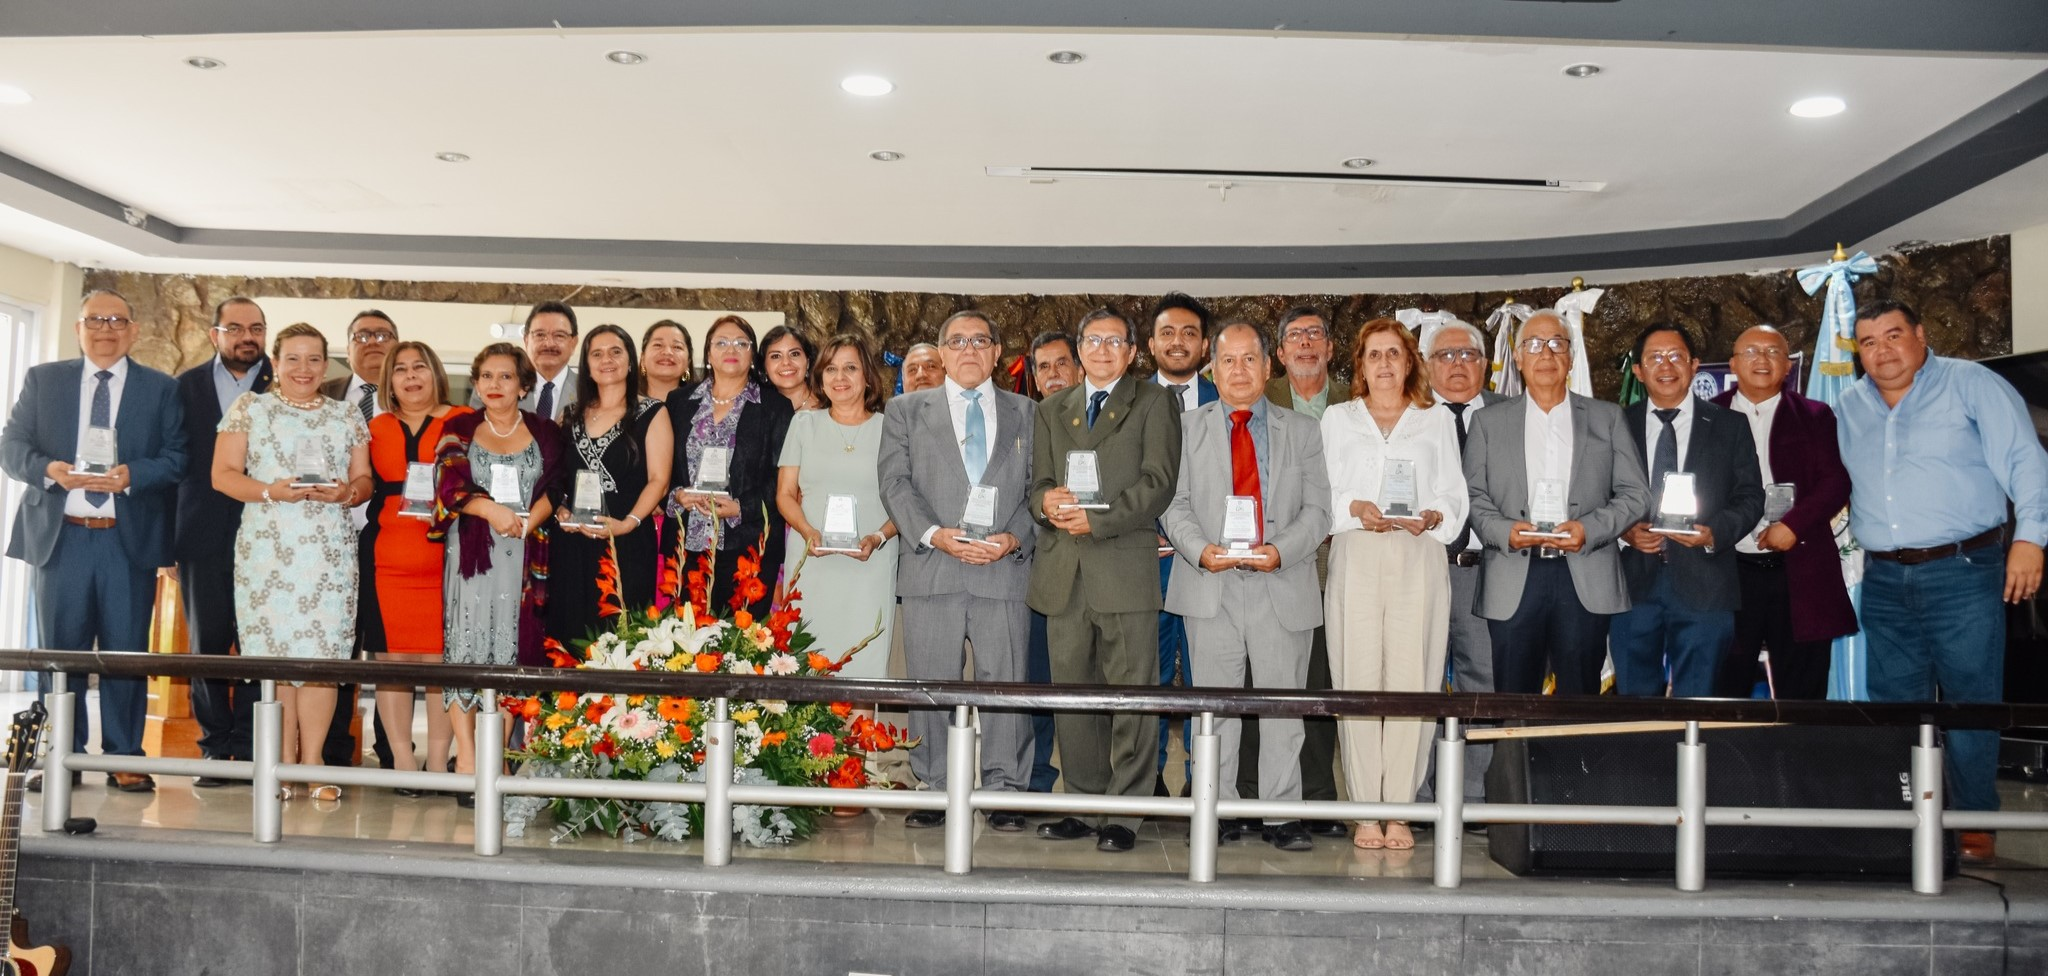
\includegraphics[width=0.9\linewidth]{autores/art12} \end{center}

La Unidad de Ejercicio Profesional Supervisado (EPS) de la Facultad de Ingeniería celebró su 50 aniversario, marcando medio siglo de contribución ininterrumpida a la formación integral de los futuros ingenieros de la Universidad de San Carlos de Guatemala (USAC).

La ceremonia conmemorativa tuvo lugar en el Colegio de Ingenieros de Guatemala, donde se rindió homenaje a docentes que han colaborado con la Unidad durante varios años, destacando su compromiso y acompañamiento en el desarrollo profesional de los estudiantes. Además, se entregaron reconocimientos a los miembros de la Junta Directiva de la Facultad de Ingeniería, como muestra de gratitud por su apoyo institucional y su papel clave en el fortalecimiento continuo de la EPS.

Durante el acto, se contó con las palabras de apertura del Decano a.i., José Francisco Gómez Rivera, y del Ing. Oscar Argueta, director de la Unidad, quienes ofrecieron una remembranza del origen y evolución del programa.

La Unidad de EPS nació en 1971 como una iniciativa de estudiantes y autoridades académicas, con la visión de transformar una formación basada únicamente en la teoría, en una experiencia educativa activa y conectada con las necesidades del país. Fue aprobada formalmente en 1973, consolidándose como una propuesta académica innovadora que fusionó el rigor técnico con el compromiso social, marcando un antes y un después en la enseñanza de la ingeniería en Guatemala.

Como parte del programa de la ceremonia, se presentaron intervenciones especiales que enriquecieron el ambiente con arte, reflexión y sentimiento, en la que resalta la del Ingeniero Silvio Rodríguez Serrano, que con profunda sensibilidad, compartió un texto de su autoría titulado «La Ceiba del EPS», inspirado en los 50 años de la Unidad. En su lectura, evocó a la Ceiba como símbolo de fortaleza, sabiduría y arraigo, haciendo un paralelismo con la labor de la EPS y el espíritu de servicio de los estudiantes epesistas. La reflexión dice así:
\begin{center}
\emph{``Caminaba bajo el cielo azul de la ciudad Universitaria,}

\emph{me llamó una voz}

\emph{desde un árbol majestuoso y gigante.}

\emph{Vi la Ceiba fuerte,}

\emph{de raíces profundas.}

\emph{Sus ramas alcanzan el firmamento,}

\emph{donde las aves encuentran su hogar,}

\emph{como una verde y serena catedral.}

\bigskip

\emph{¿Qué me querías decir?}

\emph{pregunté a la voz.}

\emph{Una figura perfecta}

\emph{que relata el sentir y el ser}

\emph{de nuestro EPS.}

\emph{Se me mostró cómo se extiendes}

\emph{cual brazo fuerte del conocimiento,}

\emph{para abrigar con diseños y soluciones}

\emph{a los espacios más necesitados de nuestra sociedad.}

\emph{por eso el ramaje me recordó}

\emph{a todas nuestras ingenierías.}

\emph{Que vengan entonces las mismas,}

\emph{y se extiendan con la savia verde de la fuerza}

\emph{por los cuatro puntos cardinales de nuestra Patria:}

\emph{La ingeniería Civil, Industrial, Mecánica,}

\emph{Química, Eléctrica, Electrónica y Ciencias y Sistemas.}

\bigskip
\bigskip

\emph{Oh grandioso EPS, sé como la grandiosa Ceiba,}

\emph{que sigue en pie aún después de las peores tormentas.}

\emph{En el crisol del tiempo infinito,}

\emph{testimonio de nuestra presencia.}

\emph{Enraíza tu espíritu de servicio en nosotros.}

\emph{y como premio del esfuerzo que realizas,}

\emph{que broten las flores en forma de guirnaldas.}

\bigskip
\bigskip

\emph{Para los valientes guerreros epesistas}

\emph{que se animaron para aceptar el reto,}

\emph{conociendo las verdades de nuestra sociedad,}

\emph{presentando soluciones}

\emph{transformando nuestro lema universitario}

\emph{``Id y enseñad a todos'',}

\emph{En ``Id y aprended de todos''.}

\bigskip
\bigskip
\bigskip
\bigskip
\bigskip
\bigskip
\bigskip
\bigskip
\bigskip

\emph{Loor a ustedes muchachos valientes,}

\emph{que se embebieron con el elixir de la experiencia,}

\emph{y se embriagaron con la práctica de la Ingeniería}

\emph{en problemas desconocidos.}

\emph{Salud a ustedes jóvenes epesistas}

\emph{Son como esas guirnaldas:}

\textbf{\emph{NUESTRO ORGULLO Y NUESTRA SATIFACCCIÓN}}

\bigskip
\bigskip

\emph{Y la sabia Ceiba sigue creciendo".}
\end{center}

\begin {flushleft}
\noindent\begin{minipage}[c]{\columnwidth}

\begin{center}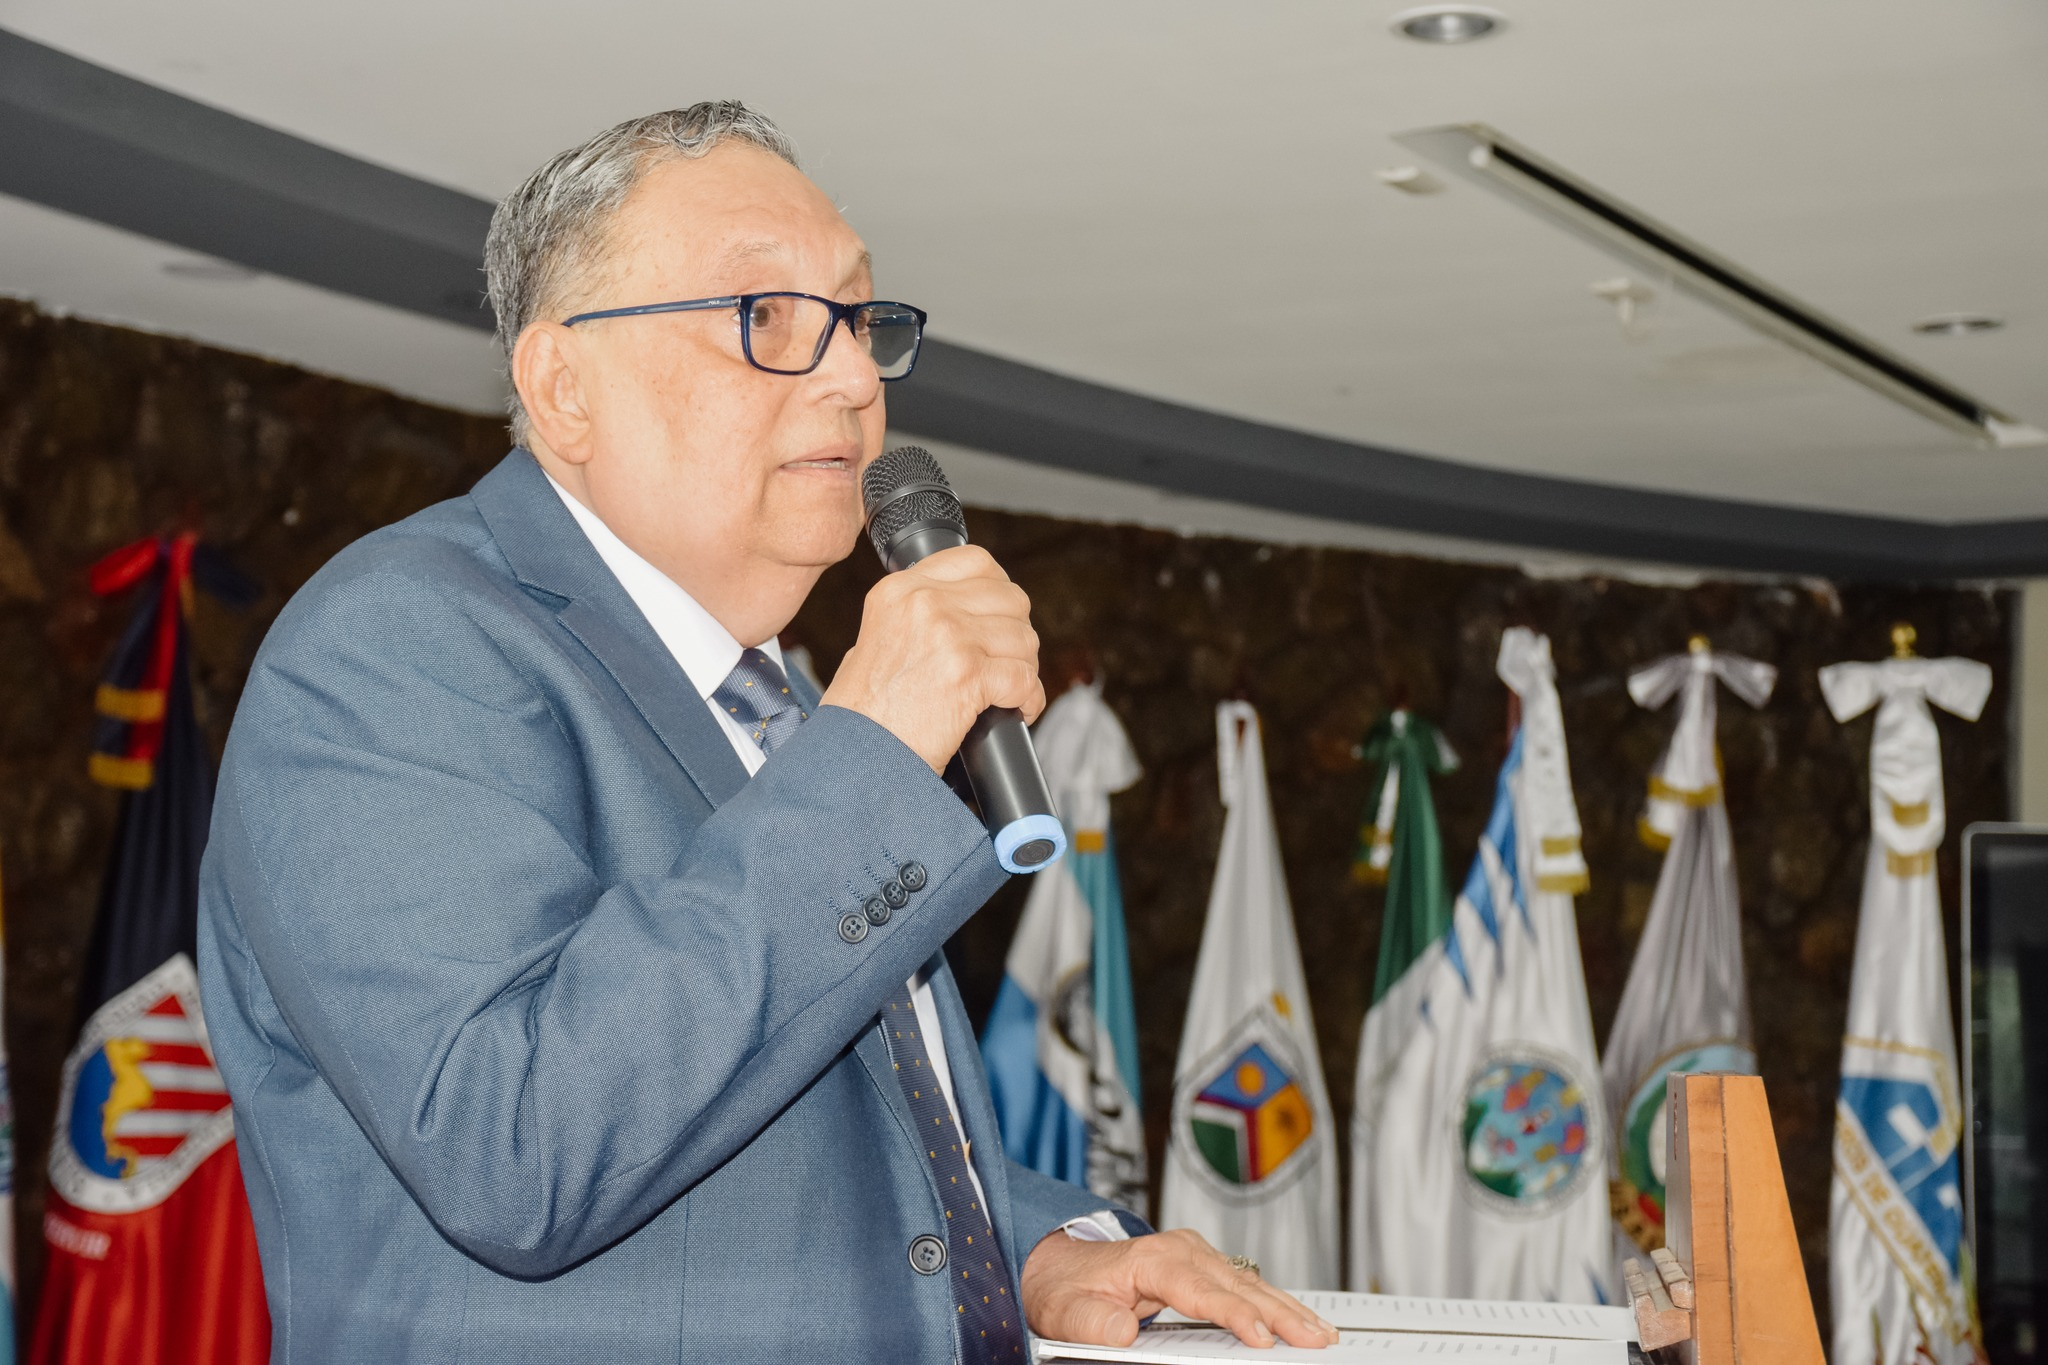
\includegraphics[width=0.6\linewidth]{imagenes_articulos/art12_01} \end{center}

\textbf{Ing. Silvio José Rodríguez Serrano}

\end{minipage}
\end {flushleft}

Desde sus inicios, la EPS ha evolucionado para responder a los desafíos sociales y tecnológicos del país, sin perder su esencia: ser el puente entre la academia y la sociedad. El Ing. Oscar Argueta Hernández, director de la Unidad de Prácticas de Ingeniería y EPS, ha destacado que el mayor aporte del programa ha sido brindar a los estudiantes la oportunidad de aplicar sus conocimientos en contextos reales, generando soluciones técnicas sostenibles y pertinentes bajo supervisión profesional.

A lo largo de cinco décadas, la EPS ha sido clave en el desarrollo de competencias profesionales, éticas y sociales en los futuros ingenieros. De cara al futuro, la Unidad proyecta la modernización de sus metodologías, mayor vinculación con sectores gubernamentales y productivos, y una expansión de sus áreas de impacto, con el firme compromiso de contribuir al desarrollo sostenible del país.

La celebración de este 50 aniversario no solo honra la historia de la EPS, sino que renueva su misión de formar ingenieros comprometidos, conscientes y preparados para transformar su entorno.

\medskip

\HRule

\medskip

\bibliography{book.bib,packages.bib}

%%%%\printindex



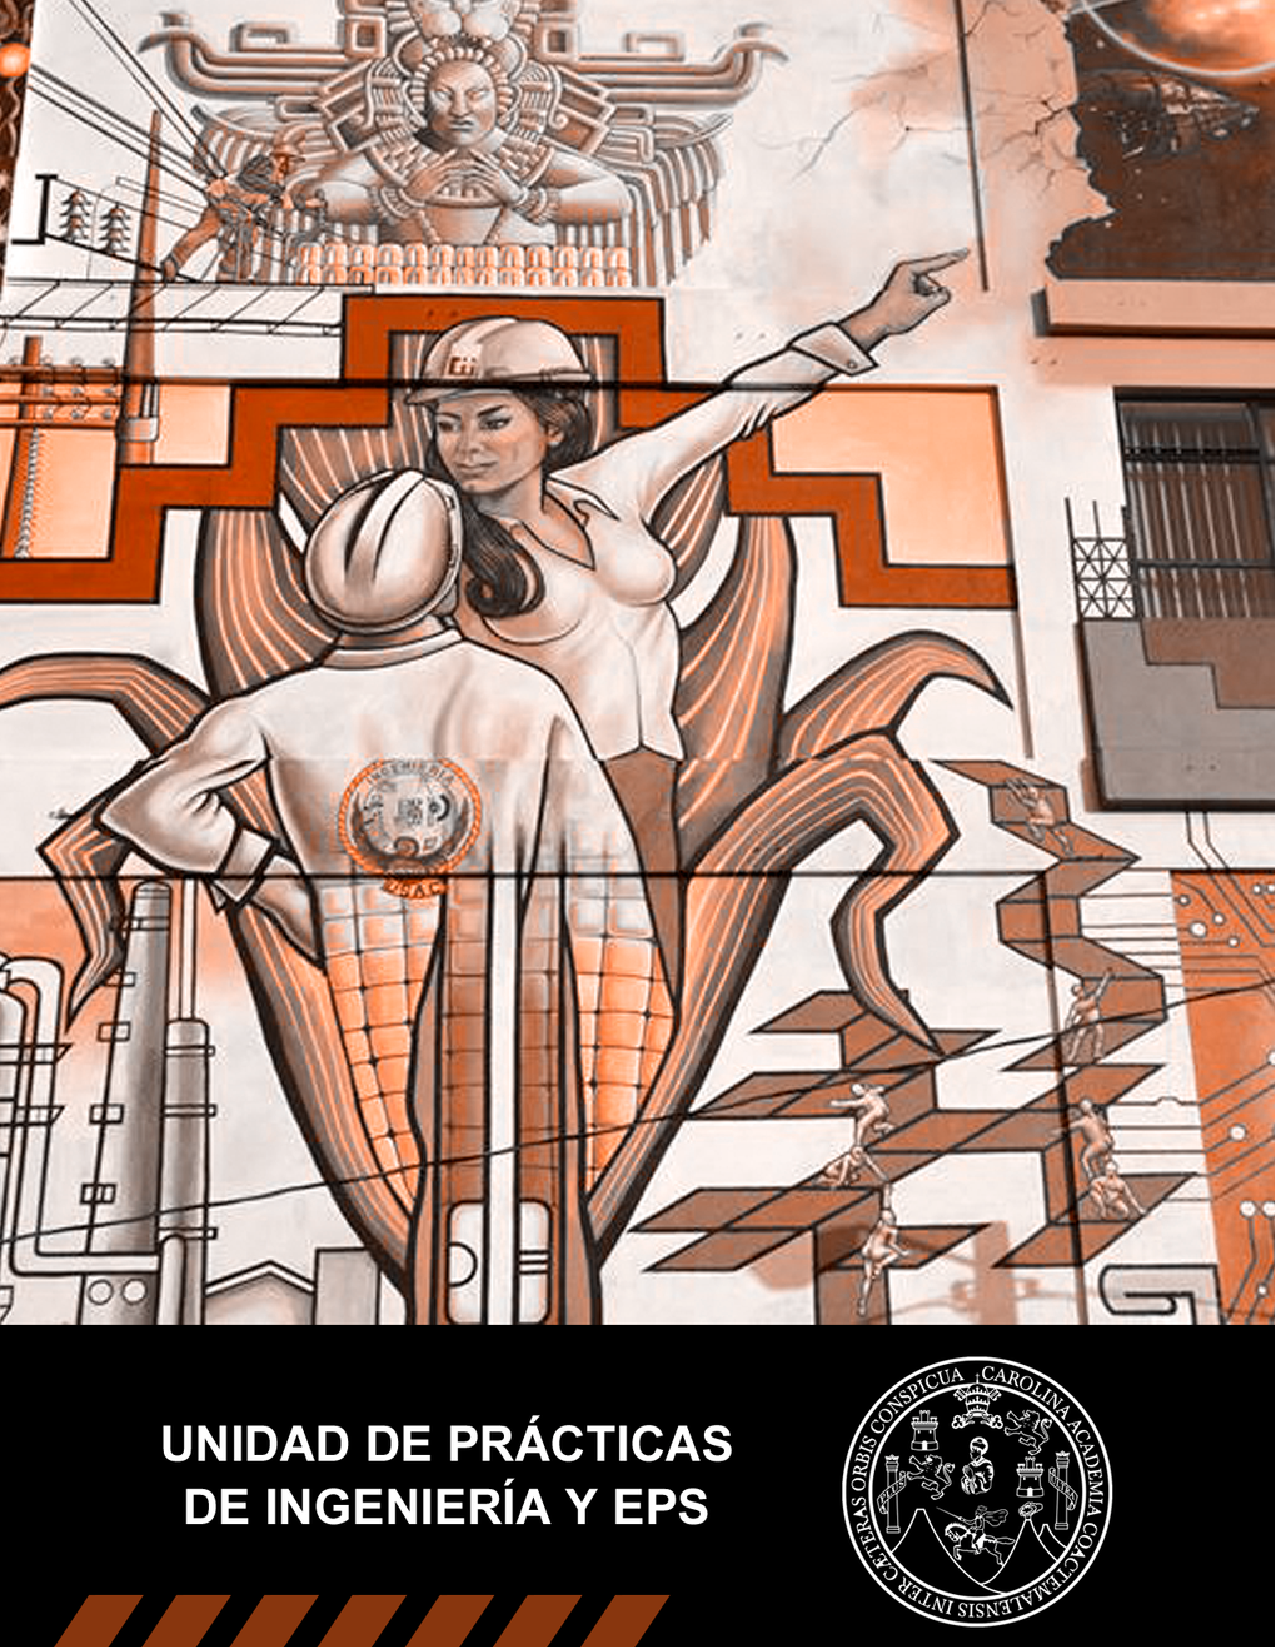
\includepdf{images/contraportada.pdf}


\end{document}
